\chapter[Solução Eletrônica]{Solução Eletrônica}

Este capítulo é voltado para o desenvolvimento do sistema eletrônico, apresentando as escolhas de projeto a partir dos requisitos técnicos. Assim, esse sistema foi dividido em 3 módulos: Módulo de Medição e Identificação, Módulo de Controle e Módulo de Visualização. Pela forma que o sistema eletrônico foi dividido os 3 módulos possuem grande dependência entre si.

\section{Módulo de Medição e Identificação}

O módulo de medição e identificação tem a funcionalidade de realizar a aquisição dos seguintes dados para uso no controle do dispositivo:

\begin{itemize}
    \item Medição:
    \begin{itemize}
        \item Temperatura;
        \item Umidade.
    \end{itemize}
    \item Identificação:
    \begin{itemize}
        \item Passagem de objetos (medicamentos e copos);
        \item Usuário por biometria;
        \item Informações do copo que está sendo depositado os medicamentos;
        \item Imagens dos medicamentos no copo para validar a entrega.
    \end{itemize}
\end{itemize}

Sendo assim, trata-se de um módulo micro-controlado conectado a vários componentes de identificação e medição, representação por diagrama na Fig. \ref{fig:modulo_medicao}. Dessa forma, os componentes foram selecionados a partir dos requisitos levantados, disponibilidade no Brasil, custos acessíveis e escala de medição compatível com a aplicação. 

\begin{figure}[H]
    \centering
    {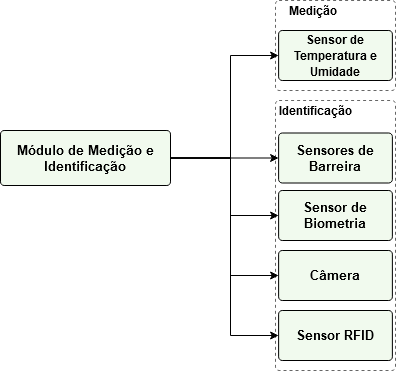
\includegraphics[width=0.5\textwidth]{figuras/eletronica/esquematicos/m_medicao.png}}
    \caption{Módulo de Medição e Identificação} 
    \label{fig:modulo_medicao}
\end{figure}


\subsection{Medição}
    \subparagraph*{$\bullet$ Sensor de Temperatura e Umidade} \hfill
    
     O uso do sensor de temperatura e de umidade foi baseado na necessidade do monitoramento constante das variáveis de temperatura e umidade relativa dentro do dispositivo. A maioria dos medicamentos sólidos precisa estar armazenada em uma faixa de temperatura e umidade relativa determinada pelo fabricante para não alterar as propriedades químicas e a integridade dos medicamentos. 
    
    Para seleção do componente, foram priorizados sensores com mais de uma funcionalidade, isto é, sensores de temperatura e umidade relativa integrados. Sendo assim, a faixa de valores para a conservação de medicamentos sólidos está entre 15 $^\circ$C e 30 $^\circ$C e a escala de umidade relativa de 40\% a 70\% \cite{Pinto_2016}. Adicionalmente, deve ser levado em consideração, para escolha de um sensor em determinada aplicação, os parâmetros de acurácia, precisão, sensibilidade e resolução \cite{webster2018measurement}. 
    
    Como os parâmetros medidos de temperatura e umidade não são unidades de mudança rápida em pequenos intervalos de tempo (sendo o menor de 1 segundo) no ambiente onde o sensor está inserido, o modelo escolhido não precisa ter uma taxa de atualização maior que 1 Hz \cite{webster2018measurement}. Entretanto, se tornou preferível escolher aqueles com maior resolução, operantes na faixa de conservação do medicamento e com precisão menor que 1 $^\circ$C para temperatura e 5\% UR para umidade relativa, a fim de diminuir a faixa de dúvida do sensor utilizado. Por fim, foi-se priorizado os sensores em um módulo comercial que entregavam os dados de forma digital em um protocolo compatível com o módulo de controle. Ou seja, saída compatível com os protocolos \textit{Inter-Integrated Circuit} (I$^2$C), \textit{Serial Peripheral Interface} (SPI), \textit{Universal Asynchronous Receiver/Transmitter} (UART), \textit{Display Serial Interface} (DSI) ou \textit{Camera Serial Interface} (CSI).
    
    Sendo assim, o sensor selecionado foi o \textbf{HTU21D}, embarcado em um módulo comercial, pelo fato de ser um sensor compatível com as faixas de captura, resolução e precisão dos dados, com preço de compra menor que R\$ 50,00,  além do sinal de saída digital no protocolo interface I$^2$C, compatível com o módulo de controle.
    
    Para este sensor, nenhum condicionamento é necessário para o sinal, por ser realizado internamente no módulo. A conexão do sensor com o módulo de controle consiste em 4 pinos: VDD, GND e duas linhas de dados para comunicação I$^2$C (SDA/SCL). Além do mais, possui resolução configurável por \textit{software}, sendo 8/12 \textit{bits} para umidade e 12/14 bits para temperatura. O módulo \textbf{HTU21D} está representado na Fig. \ref{fig:sensor_temp_umidade}, e possui as seguintes especificações:
    
    \begin{figure}[H]
        \centering
        \subfloat[][Sensor HTU21D]{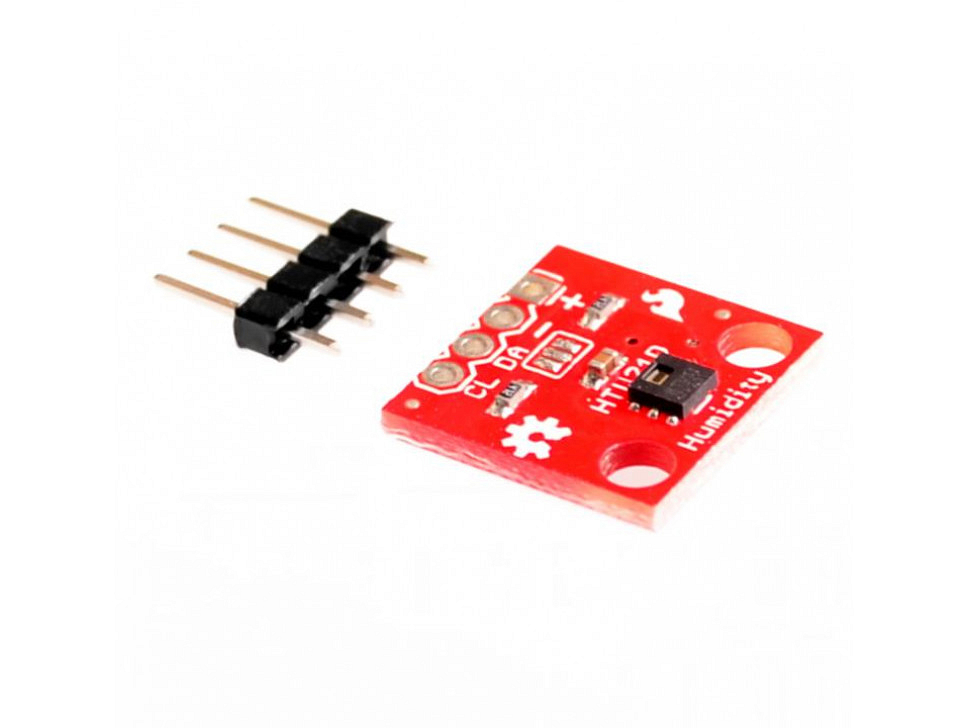
\includegraphics[width=0.3\textwidth]{figuras/eletronica/fotos_componentes/sensor_temp_umi.jpg}\label{fig:sensor_temp_umi_pic}}
        \hspace{0.1\textwidth}
        \subfloat[][Conexões do Sensor HTU21D]{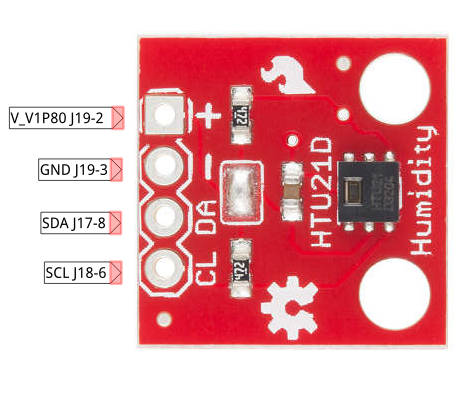
\includegraphics[width=0.3\textwidth]{figuras/eletronica/esquematicos/HTU21D.jpg}\label{fig:sensor_temp_umi_esq}}
        \caption{Sensor de Temperatura e Umidade}\label{fig:sensor_temp_umidade}
    \end{figure}
    
    \begin{itemize}
    \item[]
        \begin{itemize}
            \item \textbf{Alimentação:} 1,5 V a 3,6 V;
            \item \textbf{Consumo de corrente em medição:} 500 $\mu$A;
            \item \textbf{Faixa de medição da umidade:} 0-100\% UR;
            \item \textbf{Faixa de temperatura de medição:} -40 a 105 $^\circ$C;
            \item \textbf{Precisão da umidade (10\% a 95\% UR):}  $\pm$ 2\% UR;
            \item \textbf{Precisão da temperatura:} $\pm$ 0.3 $^\circ$C;
            \item \textbf{Interfaces de Comunicação:} I$^2$C;
            \item \textbf{Dimensões:} 15,8 x 15,6 x 2 mm;
            \item \textbf{Preço:} R\$ 18,90.
        \end{itemize}
    \end{itemize}
    
\subsection{Identificação}
    \subparagraph*{$\bullet$ Sensor Fotoelétrico} \hfill
    
    Os sensores fotoelétricos foram utilizados para detectar a passagem do medicamento sólido, tanto na saída das comportas quanto no final da zona de transição. Além disso, utilizou-se esse sensor para as seguintes detecções: presença do copo no reservatórios de copos; identificação da presença do copo em local predeterminado para o processamento de imagem; passagem do copo com medicamentos errados para o compartimento traseiro; e passagem do copo para o compartimento frontal.
    
    Assim, optou-se pela utilização do sensor de barreira, o qual o emissor e o receptor são instalados frente a frente para permitir que a luz do emissor entre no receptor. Logo, quando um objeto passa entre o emissor e o receptor, a luz que entra no receptor é interrompida ou reduzida, e assim é possível detectar a presença de um objeto, conforme as Fig. \ref{fig:sensor_infra} e  \cite{amron_photo_sensors}.
    
    \begin{figure}[H]
        \centering
        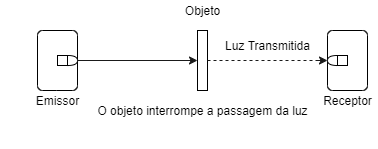
\includegraphics[width=0.6\textwidth]{figuras/eletronica/fotos_componentes/sensor_infra.png}
        \caption{Sensores de Barreira}
        \label{fig:sensor_infra}
    \end{figure}
    
    Por se tratar de um sensor de simples implementação, optou-se por fazer a implementação utilizando: um \textit{LED} emissor de infravermelho (\textbf{IR333C}), um fototransistor receptor de infravermelho (\textbf{PT333-3B}) e circuito comparador.
    
    Dessa forma, para construção do circuito do sensor fotoelétrico de barreira, deve-se determinar a resistência de polarização do LED \textbf{IR333C} e determinar a potência do resistor conforme as Eq. \ref{eq:res_LED} e \ref{eq:Pot_Res}:
    
    \begin{equation}
        R_{LED} = \frac{(V_{Fonte} - V_{LED})}{I_{LED}} = \frac{( 5 - 1,5) \hspace{0.1cm} [\text{V}]}{20 \hspace{0.1cm} [\text{mA}]} = 175 \quad [\Omega]
        \label{eq:res_LED}
    \end{equation}
    
        \begin{equation}
        P_{R_{LED}} = V_{RES} \cdot I_{LED} = 3,5 \hspace{0.1cm}
        [\text{V}] \cdot 20 \hspace{0.1cm} [\text{mA}] = 0,07 \quad [\text{W}] 
        \label{eq:Pot_Res}
    \end{equation}
    
    Consequentemente, foi selecionado o resistor de 180 $\Omega$, por se tratar de um resistor comercial. A Fig. \ref{fig:esq_sensor_barreira} mostra o esquemático do circuito, enquanto a lista subsequente descreve os itens a serem utilizados na construção.
    
    \begin{figure}[H]
    \centering
    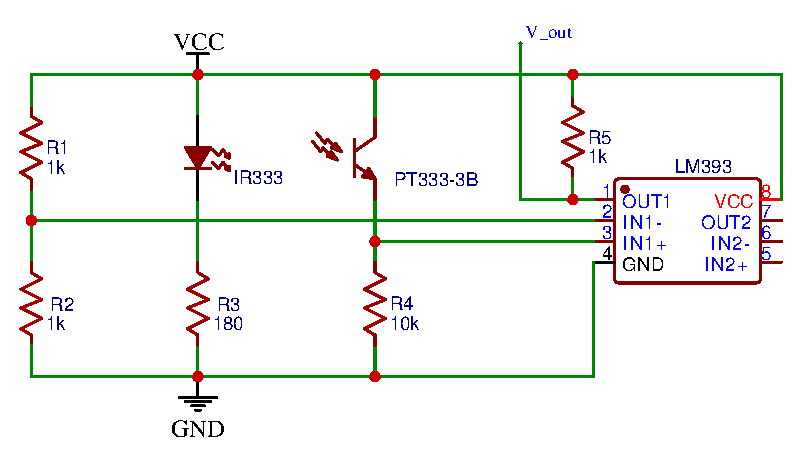
\includegraphics[scale=0.6]{figuras/eletronica/esquematicos/sensor_barreira/Schematic_Sensor_barreira.pdf}
    \caption{Esquemático do circuito do sensor fotoelétrico de barreira}
    \label{fig:esq_sensor_barreira}
    \end{figure}
    
    \begin{itemize}
    \item[ ]
        \begin{itemize}
            \item 1 LED IR333;
            \item 1 Fototransistor PT333-3B;
            \item 1 CI LM393;
            \item 1 Resistor de 180 $\Omega$;
            \item 1 Resistor de 10 k$\Omega$;
            \item 3 Resistores de 1 k$\Omega$.
        \end{itemize}
    \end{itemize}
    
    Para realizar as simulações, foi utilizado o Opto-acoplador \textbf{4N25}, o qual consiste em um CI que contém um LED emissor de infravermelho e um fototransistor NPN. Optou-se pela utilização desse componente na simulação uma vez que os valores de tensão e corrente de entrada e saída são os mesmos para os componentes selecionados \textbf{IR333} e \textbf{PT333-3B}. Entretanto, a única variação do \textbf{4N25} em relação ao LED emissor \textbf{IR333} é a corrente de entrada de 50 mA para o circuito integrado (C.I.) e 20 mA para o LED, o que pode ser corrigido na simulação pela alteração do resistor do LED.
    
    Outrossim, na simulação de acordo com a Fig. \ref{fig:sim_sensor_barreira}, foi adicionada uma sequência de pulsos na entrada do LED emissor para representar a passagem do objeto entre o emissor e o receptor. Uma vez que, com a passagem do objeto, tem-se a ausência de luz, as junções inversamente polarizadas do fototransistor não conduzem corrente elétrica, e se tem como resultado uma resistência ``infinita''. Após a passagem do objeto, ocorrerá a entrada de luz nestas junções e sua resistência diminuirá, havendo assim a condução de corrente elétrica. 
    
    Decorrida essa variação de corrente, tem-se uma consequente alteração na tensão e, dessa forma, é possível utilizar o C.I. \textbf{LM393}, que contém dois amplificadores operacionais comparadores de tensão. Por conseguinte, liga-se a entrada inversora do comparador a um par de resistores cujos valores determinam a tensão de referência. Quando o valor na entrada não-inversora for maior que o valor de referência na entrada inversora, a saída do comparador tende a 5 V. Enquanto que, quando o valor na entrada não-inversora for menor que o valor de referência na entrada inversora, a saída do comparador converge a 0 V. 
    
    \begin{figure}[H]
    \centering
    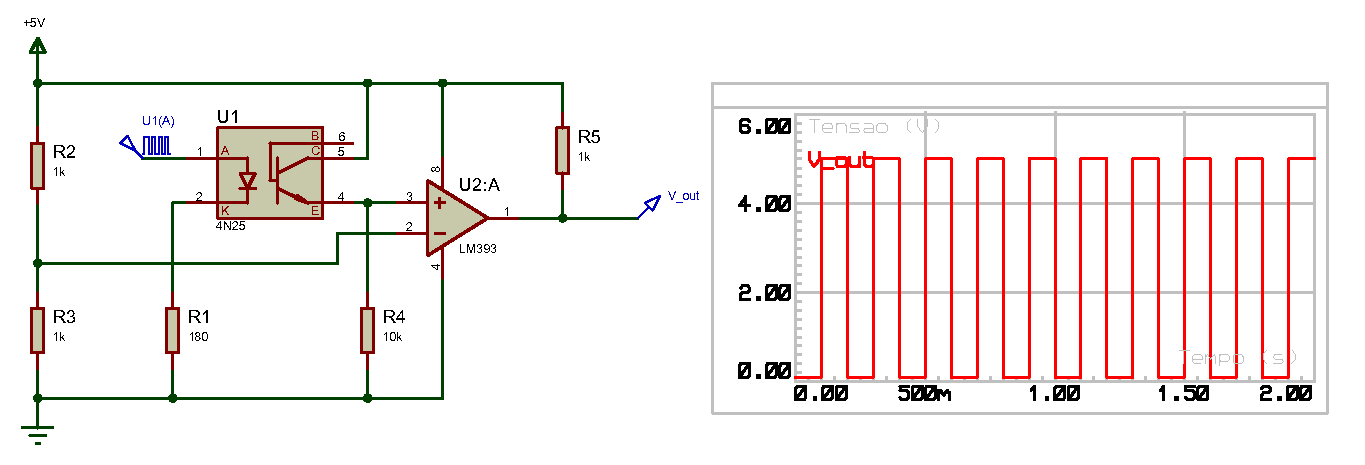
\includegraphics[scale=0.65]{figuras/eletronica/esquematicos/sensor_barreira/Sim_sensor_barreir_3.PDF}
    \caption{Simulação do Sensor Fotoelétrico de barreira}
    \label{fig:sim_sensor_barreira}
    \end{figure}
    
     Portanto, a partir dessa variação de tensão na saída, pode-se detectar a passagem do objeto, traduzindo a oscilação de 5 V e 0 V para uma representação digital ao ser conectado com o módulo de controle. Essa conexão utiliza 3 pinos: Terminal 1 é a alimentação do circuito em 5 V, Terminal 2 é o terra (em inglês \textit{Ground} - GND) e o Terminal 3 é a saída do comparador \textbf{LM393}, representado como $V_{out}$ no esquemático da Fig. \ref{fig:sim_sensor_barreira}. Como a saída $V_{out}$ é uma saída digital, ou seja, quando for 0 V, temos {bit} 0 e em 5 V temos {bit} 1, não sendo necessário o uso de um condicionamento de sinal como de conversores analógico-digital para conexão entre o sensor desenvolvido e o módulo de controle.

    Para levantamento da corrente total consumida pelo sensor de barreira é levada em consideração a corrente típica de operação para o \textit{LED} emissor ($I_{LED}$) e a corrente da fonte de alimentação para simulação na Fig. \ref{fig:sim_sensor_barreira} excluindo o IN25 ($I_{CIRCUITO}$). Como $I_{LED} =$ 20 mA e $I_{CIRCUITO} =$ 5 mA  obtemos a corrente total somando-as. Ou seja, $I_{total} = I_{LED} + I_{CIRCUITO} =$ 25 mA.  
    
    Por último, a partir da simulação, foi realizada a placa de circuito impresso conforme a Fig. \ref{fig:PCB_barreira} no apêndice \ref{app:PCB}.  

    \subparagraph*{$\bullet$ Sensor de Biometria} \hfill
    
    O funcionamento deste sensor se baseia na aquisição da impressão digital do usuário por meio de uma imagem que, posteriormente, terá suas características únicas extraídas e comparadas com um banco de dados de impressões digitais cadastradas. 
    
    Dessa forma, foi escolhido o sensor óptico de digitais \textbf{DY50}, Fig. \ref{fig:sensor_biometria}, por ser o mais comum no mercado e possuir uma metodologia validada para obtenção de digitais. Esse sensor tem a funcionalidade de legitimar o funcionário da clínica geriátrica e permitir a realização de funções que necessitam de autenticação. Assim, esse sensor é empregado para liberar o compartimento frontal para a retirada da dose medicamentosa do dispensador e também para realizar o abastecimento do estoque de medicamentos.
    
   A conexão do sensor com o módulo de controle consiste em 4 pinos, e seu esquemático consta na Fig. \ref{fig:biometria_esq}: VCC e GND para alimentação, TX e RX para a comunicação UART. O sensor de biometria \textbf{DY50} está representado na Fig. \ref{fig:biometria_fig}, e possui as seguintes especificações:
    
    
    \begin{figure}[H]
        \centering
        \subfloat[][Sensor DY50]{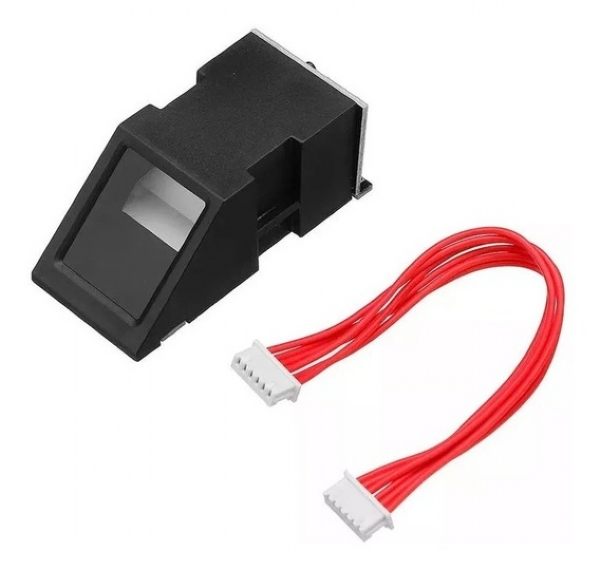
\includegraphics[width=0.35\textwidth]{figuras/eletronica/fotos_componentes/sensor_biometria.jpg}\label{fig:biometria_fig}}
        \hspace{0.1\textwidth}
        \subfloat[][Conexões do Sensor DY50]{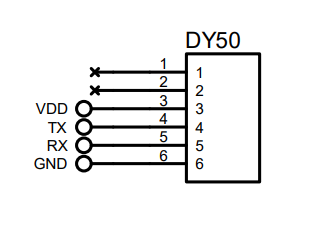
\includegraphics[width=0.35\textwidth]{figuras/eletronica/esquematicos/esq_conex_biometria.png}\label{fig:biometria_esq}}
        \caption{Sensor Biometria DY50}\label{fig:sensor_biometria}
    \end{figure}
    
    \begin{itemize}
    \item[ ]
        \begin{itemize}
            \item \textbf{Alimentação:} 3,6 V a 6 V;
            \item \textbf{Consumo de corrente máximo:} 120 $m$A;
            \item \textbf{Taxa de transmissão:} 9600, 19200, 28800, 38400, 57600 bits por segundo (bps);
            \item \textbf{Comunicação:} \textit{Transistor Transistor Logic} serial (TTL serial);
            \item \textbf{Preço:} R\$ 69,00.
        \end{itemize}
    \end{itemize}
    
    \subparagraph*{$\bullet$ Sensor de Leitura RFID} \hfill
    
    Para realizar a identificação e logística de distribuição de medicamentos para os pacientes, cada copo tem cores únicas para evitar ministração errada de doses medicamentosas entre pacientes, conforme mencionado na seção \ref{sec:copo_estrutura} da solução estrutural. Desse modo, sua identificação é necessária para determinar o copo que está recebendo a medicação. 
    
    Dado essa problemática, o sensor RFID foi escolhido para identificar o copo utilizado na separação das doses de medicamentos. Ele realiza a leitura de uma tag RFID pré-instalada e com informações de identificação (ID) exclusivas para cada cor de copo.
    
    O sensor RFID escolhido foi o com C.I. controlador \textbf{PN532}, Fig. \ref{fig:sensor_RFID}. Devido a distância máxima para leitura e escrita chegar à 70 mm e sua antena poder ser modificada e direcionada para atender as necessidades de dimensionamento do dispositivo. Este C.I. contempla um projeto de circuito com os componentes necessários para conectar uma antena, fornecido pelo fabricante. O circuito RF consiste em 8 capacitores, 2 indutores, 2 resistores e a bobina de antena simétrica, como mostrado na Fig. \ref{fig:antena_RFID}
    
    O filtro EMC reduz harmônicos de 13,56 MHz e executa uma impedância de transformação. Em seguida, o circuito para casamento de impedâncias atua como um bloco de transformação de impedância. Por último, a própria bobina da antena gera o campo magnético, e assim recebe ou envia um sinal correspondente processado pelo PN532.
    
    \begin{figure}[H]
    \centering
    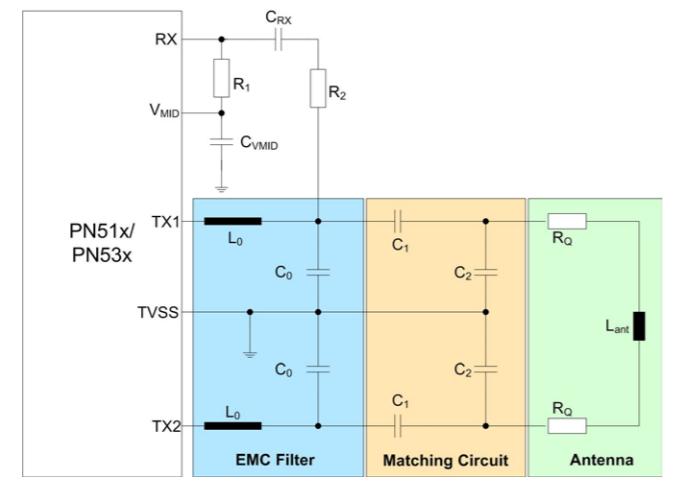
\includegraphics[scale=0.65]{figuras/eletronica/esquematicos/antena_RFID.png}
    \caption{Diagrama de blocos da parte RF}
    \label{fig:antena_RFID}
    \end{figure}

   Para simplificar o desenvolvimento foi escolhido uma solução comercial para sensor de leitura RFID com o PN532 integrado, nele acompanha uma antena seguindo o projeto do fabricante. Essa antena suporta a distância de até 70 mm para leitura e escrita em TAGs RFID compatíveis com a frequência de 13,56 MHz. Essa distância é suficiente para aplicação, por ser superior ao dobro espessura do módulo da esteira utilizada, 19,9 mm, indicada na Fig. \ref{fig:esteira} do apêndice \ref{cad_preliminar}.
   
   O sensor foi posicionado entre os módulos da esteira e poderá identificar tags RFID com uma distância de 50-55mm. Temos também que os módulos da esteira são feitos de plástico, não ocorrendo problemas em relação a interferência na posição onde foi definido. A tag RFID fica localizada na parte inferior do copo. Sendo possível ler a informação de identificação (ID) do copo independentemente da face virada para o sensor.
   
   A conexão do sensor de leitura RFID com o módulo de controle consiste em 4 pinos, esquemático na Fig. \ref{fig:sensor_RFID_esq}: VCC, GND, SDA e SCL, que são duas linhas de dados para comunicação I$^2$C. O componente, possui as seguintes especificações:
    
    \begin{itemize}
    \item[ ]
        \begin{itemize}
            \item \textbf{Alimentação:} 5 V;
            \item \textbf{Interfaces de Comunicação:} I$^2$C, SPI e \textit{High Speed UART} (HSU);
            \item \textbf{Distância máxima de leitura/gravação:} 70 mm;
            \item \textbf{Preço:} R\$ 33,99.
        \end{itemize}
    \end{itemize}
    
\begin{figure}[H]
    \centering
    \subfloat[][Sensor de leitura RFID PN532]{
    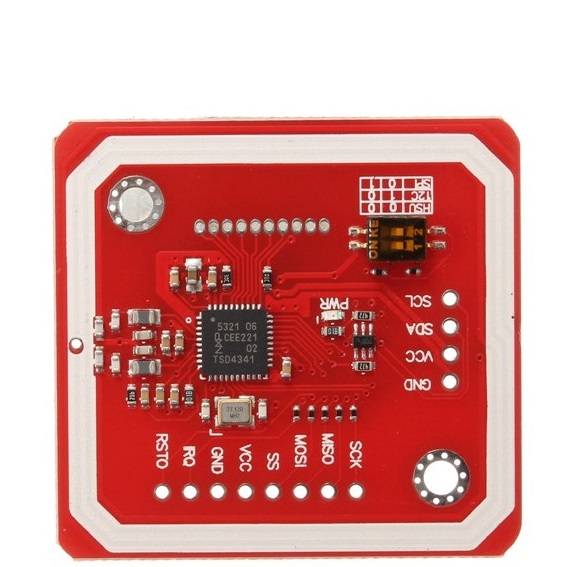
\includegraphics[width=0.2\textwidth]{figuras/eletronica/fotos_componentes/sensor_RFID.jpg}
    \label{fig:sensor_RFID}}
    \hspace{0.05\textwidth}
    \subfloat[][Conexões do módulo PN532]{
    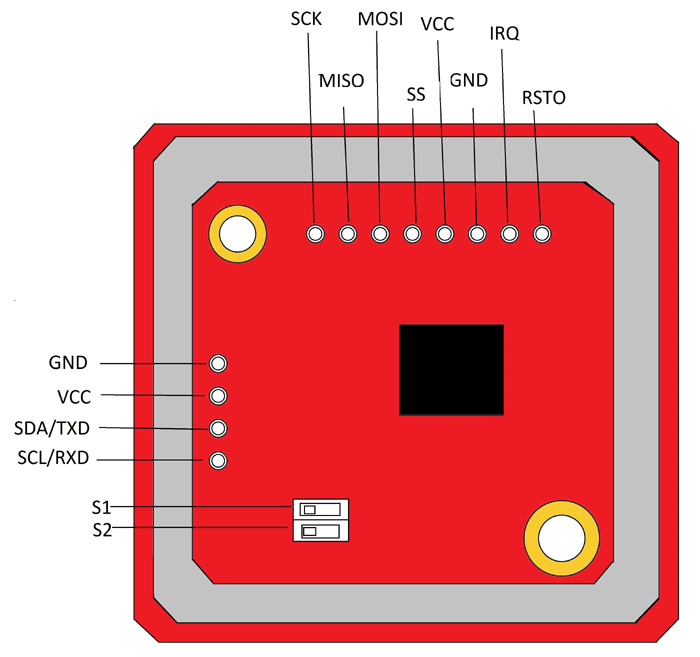
\includegraphics[width=0.2\textwidth]{figuras/eletronica/esquematicos/pinos_RFID.png}
    \label{fig:sensor_RFID_esq}}
    \caption{Módulo PN532}\label{fig:modulo_RFID}
\end{figure}

    Para escolha da \textit{tag} RFID, primeiro deve ser observado se ela é compatível para o tipo de frequência do sensor RFID utilizado, neste caso 13,56 MHz. Em seguida, deve-se ter atenção para atender as dimensões e formato do copo utilizado. Pelas cotagens descritas na Fig. \ref{fig:copo} do apêndice \ref{cad_preliminar}, copo tem base com 55 mm de diâmetro e 1,5 mm de espessura. Por fim, é necessário ser compatível para uma distância mínima de 50 mm de leitura e escrita.
   
    Seguindo a metodologia descrita, foi escolhido a \textit{Tag} etiqueta RFID 13,56 MHz, representado na Fig. \ref{fig:etiqueta_rfid}. Ela tem diâmetro de 25 mm, menor que a base do copo, e suporta uma distância de comunicação de 50 mm, suficiente para aplicação.

    \begin{figure}[H]
        \centering
        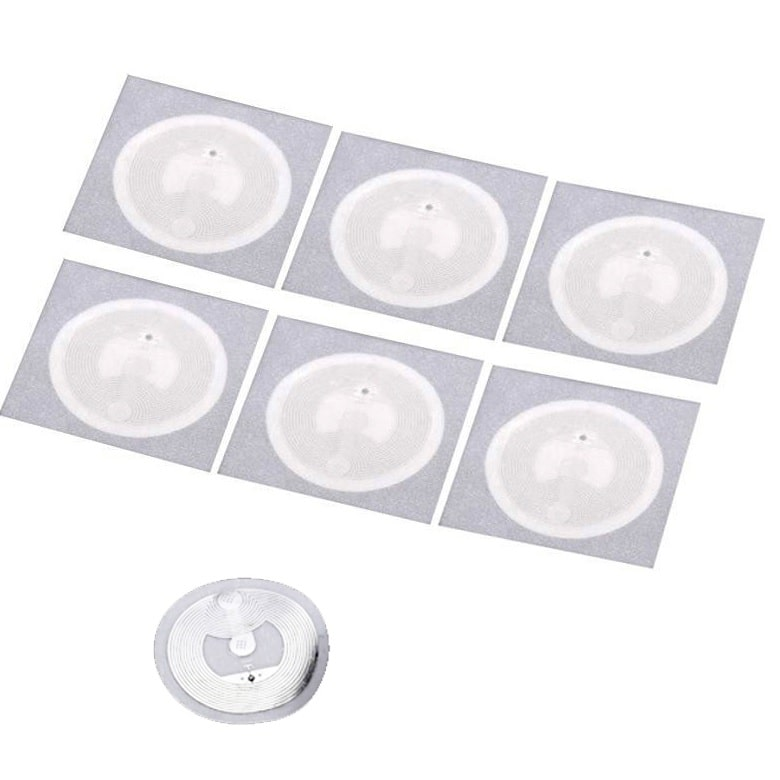
\includegraphics[width=0.25\textwidth]{figuras/eletronica/fotos_componentes/etiqueta_rfid.jpg}
        \caption{Tag etiqueta RFID 13,56 MHz}
        \label{fig:etiqueta_rfid}
     \end{figure}
    
    \subparagraph*{$\bullet$ Câmera para Processamento de Imagens} \hfill 
    
    A câmera foi escolhida para realizar a captação visual dos comprimidos. A imagem captada é processada pelo módulo de controle para identificar a quantidade e classificar o tipo de medicamento no copo, detalhado na Sec. \ref{sec:processamento_imagens}. Essa informação é usada como medida de segurança onde a doses identificadas com as quantidades erradas do esperado são descartadas. Sendo as identificadas com erro direcionadas para porta traseira do equipamento e emitido um alerta na interface do dispositivo. 
    
    A câmera escolhida foi a \textbf{OV5647}, Fig. \ref{fig:OV5647_pic}, por apresentar sensor com capacidade de gerar imagens de até 2592x1944 pixeis e preço acessível no Brasil. Ela utiliza o protocolo \textit{Camera Serial Interface} (CSI) para transmitir dados, sendo um padrão compatível para integração com o módulo de controle. Para realizar a conexão entre a câmera e o módulo de controle, especificamente o microprocessador utilizado, emprega-se um cabo \textit{flat} de 15 canais compatível com o soquete \textit{Zero Insertion Force} (ZIF) presente tanto no microprocessador como no módulo com a câmera \textbf{OV5647}, representação esquemática na Fig. \ref{fig:OV5647_esq}. O componente apresenta as seguintes características:
    
    \begin{itemize}
    	\item[] 
    	\begin{itemize}
     		\item \textbf{Sensor:} OV5647
    		\item \textbf{Resolução:} 5 MP (2592x1944 pixeis)
    		\item \textbf{Abertura:} f1.8
    		\item \textbf{Comprimento focal:} 3.6mm (ajustável)
    		\item \textbf{Dimensões do visor:} 25 x 24 x 23,5 mm
    		\item \textbf{Interfaces de Comunicação:} CSI
    		\item \textbf{Preço:} R\$ 69,90.
    	\end{itemize}
    \end{itemize}
    
    \begin{figure}[H]
    \centering
    \subfloat[][Câmera OVN5647 com lente]{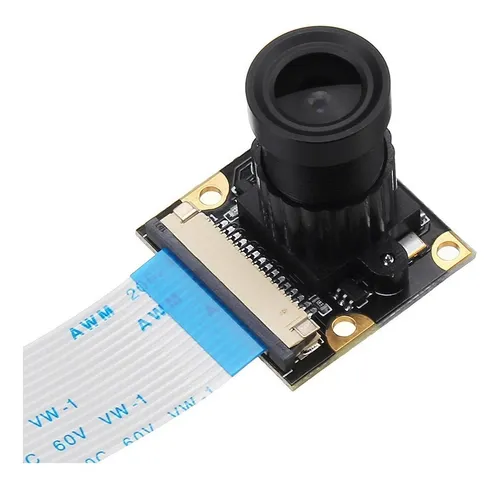
\includegraphics[width=0.25\textwidth]{figuras/eletronica/fotos_componentes/OV5647.png}\label{fig:OV5647_pic}}
    \hspace{0.1\textwidth}
    \subfloat[][Conexões CSI da Câmera OVN5647]{
    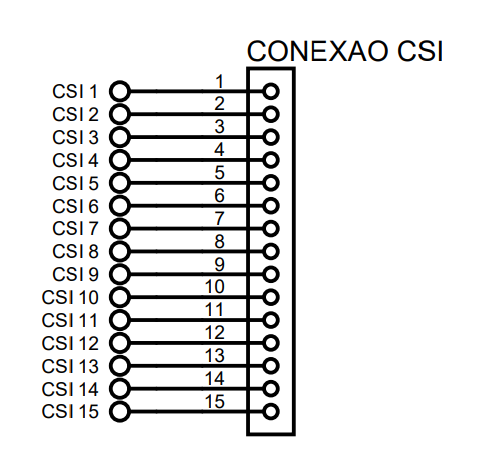
\includegraphics[width=0.25\textwidth]{figuras/eletronica/esquematicos/esq_conex_csi.png}\label{fig:OV5647_esq}}
    \caption{Câmera OV5647 - 5MP}\label{fig:camera_process}
    \end{figure}
    
\section{Módulo de Visualização}
    
    O módulo de visualização é onde o usuário poderá visualizar algumas informações úteis de funcionamento e gestão do dispositivo e interagir com essa interface usando as teclas de interação. Nele estão contidos um visor e um teclado para interface com o usuário conforme representado no diagrama da Fig. \ref{fig:modulo_visualizacao}.
    
    \begin{figure}[H]
    \centering
    {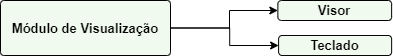
\includegraphics[width=0.6\textwidth]{figuras/eletronica/esquematicos/m_visualizacao.png}}
    \caption{Módulo de visualização} 
    \label{fig:modulo_visualizacao}
\end{figure}
    
    No apêndice \ref{app_telas_display} consta o \textit{mockup} desenvolvido para as telas presentes na interface.
    
        \subparagraph*{$\bullet$ \textbf{Visor}} \hfill
        
        Existem diversas tecnologias de visor disponíveis no mercado que podem ser utilizadas no projeto. Para delimitação do visor, foi levado em consideração compatibilidade do protocolo de comunicação com sistema embarcado escolhido, tamanho da visor, tecnologia de visor para visualização nas cores RGB e preço relativo. Sendo assim, foi escolhido o visor tipo LCD TFT de 3,2'' com as seguintes características:
        
        \begin{itemize}
        	\item[ ] 
        	\begin{itemize}
        		\item \textbf{Visor:} Tipo LCD TFT 3,2'' 
        		\item \textbf{Controlador:} ILI9341
        		\item \textbf{Resolução:} 240x320 píxeis;
        		\item \textbf{Dimensões do visor:} 48,60 x 64,80 mm
        		\item \textbf{Interfaces de Comunicação:} SPI
        	\end{itemize}
        \end{itemize}
        
        \begin{figure}[H]
        \centering
        \subfloat[][Visor tipo LCD TFT]{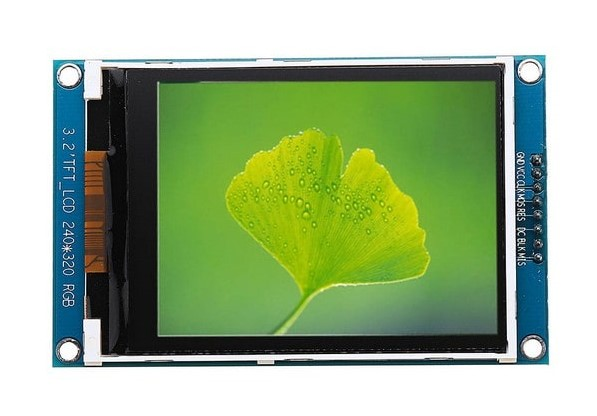
\includegraphics[width=0.4\textwidth]{figuras/eletronica/fotos_componentes/Display-LCD-TFT-3.2-240x320-6.jpg}\label{fig:LCD_pic}}
        \hspace{0.1\textwidth}
        \subfloat[][Conexões do visor LCD - Protocolo SPI]{
        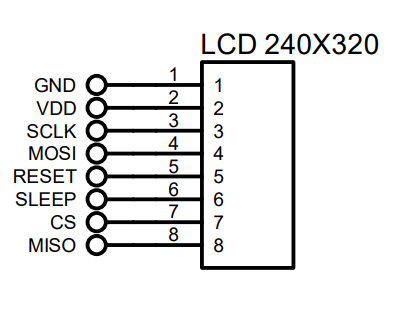
\includegraphics[width=0.365\textwidth]{figuras/eletronica/esquematicos/esq_lcd_320.png}\label{fig:LCD_esq}}
        \caption{Visor tipo LCD TFT 240x320}
        \label{fig:display_lcd}
        \end{figure}
        
        
        
        \subparagraph*{$\bullet$ \textbf{Teclado}} \hfill
        
        A utilização de uma matriz de botões é necessária para o usuário do dispositivo poder interagir com os menus de opções disponíveis no visor de visualização. Neste caso, foi preferível o uso de botões, uma vez que todos os cadastros de medicação, pacientes e enfermeiros serão realizados pelo aplicativo, e a interação no dispositivo é limitada a funções básicas, como configurações internas do dispositivo e quando há falta de internet. 
        
        
        Sendo assim, será usado uma configuração de arquitetura chamada de matriz de botões, especificamente uma solução comercial \textit{AdKeypad} com 5 botões como na Fig. \ref{fig:keypad_ft}.
        
        \begin{figure}[H]
          \centering
          \begin{minipage}[b]{0.3\textwidth}
            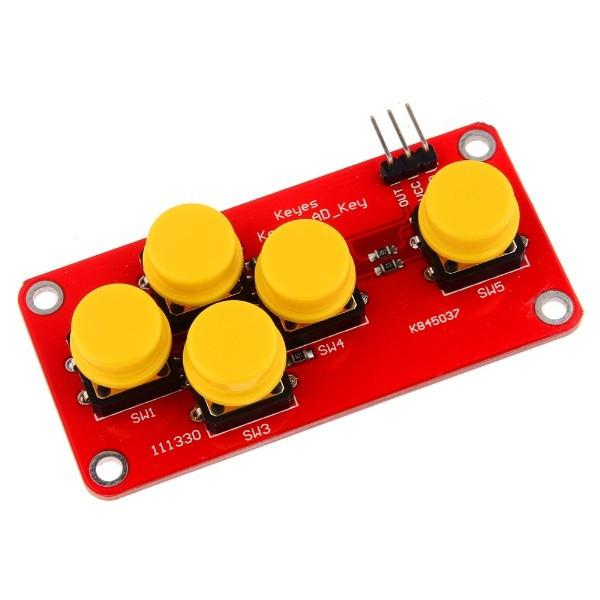
\includegraphics[width=\textwidth]{figuras/eletronica/fotos_componentes/adkeypad.jpg}
            \caption{\textit{AdKeypad} com 5 botões}
            \label{fig:keypad_ft}
          \end{minipage}
          \hspace{2cm}
          \begin{minipage}[b]{0.295\textwidth}
            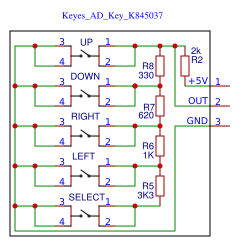
\includegraphics[width=\textwidth]{figuras/eletronica/esquematicos/adkeypad_schematic.png}
            \caption{Esquemático \textit{AdKeypad}}
            \label{fig:keypad_esq}
          \end{minipage}
        \end{figure}
        
        Analisando o circuito esquematizado na Fig. \ref{fig:keypad_esq}, pode-se calcular a saída de tensão do circuito dependendo do tipo de tecla que é clicada. O circuito se comporta como vários divisores de tensão, onde a resistência varia de acordo com a tecla que é clicada. Assim, obtemos a Eq. \ref{eq:teclado}, que representa o cálculo da tensão $V_{out}$ seguindo as entradas e saídas da Fig. \ref{fig:keypad_esq}.
        
        \begin{equation}\label{eq:teclado}
            V_{out} = \frac{R_{EQ}}{R_2 + R_{EQ}} \cdot V_{in} \quad [\text{V}]
        \end{equation}
        
        Onde $V_{in}$ é a tensão de alimentação (5 V), $R_2$ é o resistor de 2 k$\Omega$ e $R_{EQ}$ é a soma dos resistores $R_8$, $R_7$, $R_6$ e $R5$, dependendo da tecla que está sendo clicada. Sendo assim, temos o resultado de $V_{out}$ na Tab. \ref{tab:teclado}.
        
        \begin{table}[!htb]
        \centering
        \caption{Resultado para tensão $V_{out}$}
        \label{tab:teclado}
        \begin{adjustbox}{max width = \textwidth}
            \begin{tabular}{|l|c|c|c|}
                \hline
                \rowcolor[HTML]{A8DADC}
                \textbf{Tecla} & $R_2$ [k$\Omega$] & $R_{EQ}$ [$\Omega$] & $V_{out}$ [V] \\ \hline
                \textit{CIMA} & 2 & x & 0 \\ \hline
                \textit{BAIXO} & 2 & 330  & 0,708 \\ \hline
                \textit{DIREITA} & 2 & 950 & 1,610 \\ \hline
                \textit{ESQUERDA} & 2 & 1950 & 2,468 \\ \hline
                \textit{SELECIONA} & 2 & 5250 & 3,621 \\ \hline
            \end{tabular}
        \end{adjustbox}
        \end{table}
            
        Sua comunicação com microcontrolador é do tipo analógica, fazendo com o que o microcontrolador necessite de uma entrada com conversor analógico digital, para que seja realizada a leitura dos dados provenientes do teclado. 
        Conforme o esquemático na Fig. \ref{fig:keypad_esq}, pode-se observar que existe apenas um pino de dados (2) para esse teclado. O módulo de controle irá interpretar qual botão foi pressionado a partir do sinal digital resultante da conversão analógica digital da tensão de saída, determinada na Tab. \ref{tab:teclado}, no pino de dados (2). 
    
\section{Módulo de Controle}

O módulo de controle realiza o processamento dos dados coletados pelo módulo de medição e identificação, o envio e recepção de comandos do módulo de visualização e controla os atuadores do dispositivo. Além disso, é por onde comandos são recebidos e enviados  no \textit{Back-end} - nome que representa a parte da arquitetura de software que interage com o módulo de controle. 

O principal componente do módulo de controle é o computador de placa única (SBC), com outros para auxilia-lo conforme representado no diagrama da Fig. \ref{fig:modulo_controle}.

% \vspace{0.5cm} % formatação

\begin{figure}[H]
    \centering
    {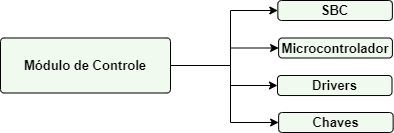
\includegraphics[width=0.6\textwidth]{figuras/eletronica/esquematicos/m_controle.png}}
    \caption{Módulo de Controle} 
    \label{fig:modulo_controle}
\end{figure}

\subsection{Sistema Embarcado}\label{sec:sistema_embarcado}
    \subparagraph*{$\bullet$ Computador de Placa Única}  \hfill
    
    A utilização de um computador de placa única (em inglês \textit{Single Board Computers} - SBCs) se dá pela necessidade desse componente desempenhar várias funções que necessitam do suporte de um computador com sistema operacional, realizando  operações para o sistema eletrônico como: Processamento de imagens dos medicamentos; Interface gráfica do módulo de visualização; Captura de dados de múltiplos sensores; Controle dos atuadores.
    
    Também é necessário que a SBC utilizada tenha suporte a protocolos de comunicação I$^2$C, \textit{SPI}, \textit{UART} e \textit{CSI}, entre os módulos de medição e identificação, visualização e o módulo de controle. Principalmente, por conter pinos GPIO para realizar a conexão física desses protocolos. Além do mais, é necessário que o sistema operacional escolhido tenha suporte as ferramentas e algoritmos de comunicação com as arquiteturas usadas na área de Software.
    
    Após uma análise de vários modelos, comparando principalmente os componentes integrados como processador central (CPU), processador gráfico (GPU), tipo de memória RAM, quantidade de memória RAM, periféricos embarcados (tipo USB, módulo Wi/Fi, internet) e o preço relativo praticado em fornecedores no Brasil, foi escolhido a \textbf{\textit{Raspberry Pi }4 B} com \textbf{4 GB DDR4}. 
    
    A \textit{Raspberry Pi} 4 tem suporte em \textit{hardware} para os protocolos de comunicação suportados para comunicação entre os componentes do módulo de controle e sensores específicos do módulo de medição e identificação. Ou seja, em seu GPIO há conexão da comunicação I$^2$C, \textit{SPI}, \textit{UART}, sendo que, para o protocolo \textit{CSI}, é utilizado o soquete ZIF de 15 pinos na parte traseira da placa. 
    
    O armazenamento será suportado em hardware pela \textit{Raspberry Pi}, sendo empregado o cartão de memória chamado em inglês de \textit{Secure Digital Card} (SD Card). Para o tamanho do cartão de memória, foi selecionado o de 32 Gb, já que não serão  armazenadas as imagens usadas no processamento de imagem e o banco de dados não armazena um grande volume de dados, apenas arquivos de Mbs e Kbs. Por fim, foi avaliado as especificações da velocidade de leitura e escrita do SD card em relação ao preço final. 
    
    Sendo assim, foi escolhido o SD Card \textbf{SanDisk Extreme} com \textbf{32 GBs} de armazenamento e especificação de leitura em até 100 MB/s e escrita de 90 MB/s. Além de atender os requisitos, essa escolha foi baseada em um comparativo de velocidade realizado pela imprensa especializada aliada ao preço em fornecedores locais \cite{sdcard_benchmark}. 
    
    Para o sistema operacional, foi escolhido o \textit{Ubuntu Server} 18.04.05 LTS por ser uma versão lançada em 2018 no mercado e pelo seu ciclo de vida terminar em Abril de 2023. Assim, o ciclo de vida representa a data final em que a versão do sistema operacional para de receber suporte oficial da comunidade \textit{Ubuntu} para atualizações de segurança e novidades. Esses sistema operacional suporta todas as bibliotecas utilizadas para desenvolvimento da comunicação e controle dos módulos do sistema eletrônico e da solução de software.
    
    \newpage 
    
    \subparagraph*{$\bullet$ Microcontroladores} \hfill
    
    Segundo \cite{morton2005pic}, para escolha do microcontrolador, primeiro deve ser realizado um rascunho do projeto, observando o que será feito e o que o microcontrolador deve fazer. O próximo passo é elaborar um diagrama do circuito ou representação similar, vendo em particular todas as entradas e saídas necessárias para se conectar com o microcontrolador e atender aos requisitos do projeto, sendo um dos principais fatores de escolha devido a limitação de porta que cada microcontrolador possui. Como, por exemplo, PIC16F54 tem até 12 pinos entrada/saída (em inglês \textit{input/output} - I/O) e a PIC16F57 até 20.
    
    Com a metodologia escolhida temos que os microcontroladores serão utilizados para direcionar dados do módulo de medição e identificação para o SBC e o mesmo enviar dados de controle para os atuadores. Para direcionamento desses dados entre os microcontroladores e o SBC escolhido (\textit{Raspberry Pi} 4), foi determinado o uso do protocolo I$^2$C, sendo assim um requisito para escolha do microcontrolador.
    
    Para determinação da quantidade de pinos, primeiro deve-se listar a quantidade de cada componente conectado aos microcontroladores e os pinos necessários para cada unidade, excluindo pinos de alimentação como +5 V e GND, e observando se os pinos utilizados atendem ao modo como o dado vem do sensor, ou seja, se é digital ou é necessário o uso de uma porta com conversão analógico-digital. Na Tab. \ref{tab:pinos_microcontrolador} está a compilação da quantidade total de pinos necessários.
    
    \begin{table}[!htb]
    \centering
    \caption{Levantamento da quantidade de pinos}
    \label{tab:pinos_microcontrolador}
    \begin{adjustbox}{max width = \textwidth}
        \begin{tabular}{|L{5cm}|C{2cm}|C{2cm}|C{2cm}|C{2cm}|C{2cm}|}
            \hline
            \rowcolor[HTML]{A8DADC}
            \textbf{Componente} & \textbf{Quantidade} & \textbf{Pinos (unid.)} &  \textbf{Tipo} & \textbf{Pinos (Total)}  \\ \hline
              Sensor de Barreira & 30 & 1  & I/O & 30
             \\ \hline
             Chave Micro \textit{Switch} & 33 & 1 & I/O & 33
            \\ \hline
             Teclado & 1 & 1 & Analógico & 1
            \\ \hline
               \textit{Driver} A4988 & 5 & 7 & I/O & 35
             \\ \hline
               \textit{Driver} IRF520N & 33 & 1 & I/O & 33
             \\ \hline
               \textit{Driver} Ponte H L298 & 1 & 2 & I/O & 2
             \\ \hline
             \rowcolor[HTML]{F1FAEE}
             \multicolumn{4}{|l|}{\cellcolor[HTML]{F1FAEE}Total} & 133 \\
             \hline
        \end{tabular}
    \end{adjustbox}
\end{table}
    Sendo levado em consideração que o visor LCD, o sensor de biometria DY50, o sensor RFID PN532, o sensor de temperatura e umidade HTU21D e a câmera não se conectam aos microcontroladores.
    
    Analisando a Tab. \ref{tab:pinos_microcontrolador}, pode-se concluir que os componentes com maior quantidade são os sensores de barreira (30 un.), as chaves (33 un.) e os \textit{drivers} IRF520N(33 un.), totalizando 95 componentes. Como o controle foi desenvolvido para que a medição ou controle para os componentes de mesmo tipo não seja paralela, é possível simplificar como eles são conectados o módulo de controle. A descrição do controle se encontra na seção \ref{sec:rede_petri}. Desse modo, pode-se utilizar multiplexadores e demultiplexadores (MUX/DEMUX) para diminuir a quantidade de portas de I/O conectadas de sensores de barreira, chaves e \textit{drivers} IRF520N com o microcontrolador. Sendo assim, foi escolhido MUX/DEMUX 8x1, especificamente pelo uso do CI CD4051. 
    
    O CD4051 é um C.I. de multiplexação ou demultiplexação com 13 pinos, dos quais: 
    
    \begin{itemize}
    	\item[]
    	\begin{itemize}
    		\item 8 pinos de entradas/saídas;
    		\item 1 pino de saída/entrada;
    		\item 3 pinos para chaveamento de qual dos oito canais são as saídas;
    		\item 1 pino \textit{ENABLE} que desliga o funcionamento do C.I.
    	\end{itemize}
    \end{itemize}
    
    
    Levando em consideração os 13 pinos de um MUX/DEMUX, foi calculado a razão de redução de pinos. Foi levado em consideração que, para o mesmo tipo de componente, é utilizada a quantidade mais próxima de MUX/DEMUX com relação a quantidade total do componente, sem deixar sobrar portas entr deada ou saída no MUX/DEMUX. Em seguida, foi considerado que os 3 pinos de chaveamento são conectados aos mesmos 3 pinos no microcontrolador, independente da quantidade utilizada de C.I.s. E os pinos de saída/entrada do MUX/DEMUX e \textit{ENABLE} tem conexão individual no multiplexador. Por fim, calculamos a razão de redução pela Eq. \ref{eq:reducao_pins}.
    
    \begin{equation}\label{eq:reducao_pins}
        \text{Razão de Redução de Pinos (RRP)} = \frac{\text{Quantidade final}}{\text{Quantidade Inicial}}
    \end{equation}
    
    Onde: Quantidade final é o total de pinos conectados ao microcontrolador após o uso dos MUX/DEMUX 8x1 e; Quantidade inicial é o total de pinos conectados determinado na Tab. \ref{tab:pinos_microcontrolador}. Seguindo a metodologia descrita, e aplicando a Eq. \ref{eq:reducao_pins} para os 3 componentes com maior quantidade, obtemos:
    
    \begin{itemize}
        \item \textbf{Sensores de Barreira:} 30 unidades, sendo 24 conectadas a 3 multiplexadores (necessário $3 + 3\cdot2 = 9$ pinos) e 6 diretamente no microcontrolador. 
        
        $RRP = \frac{(9 + 6)}{30} = 0.5$
        
        \item \textbf{Chaves tipo Micro \textit{Switch}:} 33 unidades, sendo 32 conectadas a 4 multiplexadores (necessário $3 + 4\cdot2 = 11$ pinos) e 1 diretamente no microcontrolador. 
        
        $RRP = \frac{(11 + 1)}{33} = 0.36$
        
        \item \textbf{\textit{Driver} IRF520N:} 33 unidades, sendo 32 conectadas a 4 multiplexadores (necessário $3 + 4\cdot2 = 11$ pinos) e 1 diretamente no microcontrolador. 
        
        $RRP = \frac{(11 + 1)}{33} = 0.36$
        
    \end{itemize}
    
    Recalculando o total de pinos necessários nos microcontroladores, ocorreu uma redução de 96 para 39 para os 3 componentes de maior quantidade (sensores de barreira, chaves e \textit{driver} IRF520N). 
    
    Analisando o \textit{driver} A4988, usado para os motores de passo, é necessário um total de 35 pinos. Com a funcionalidade de cada conexão explicitada na seção \ref{sec:eletronica_drivers_passo}, pode-se simplificar sua conexão aos microcontroladores, pois apenas um vai funcionar por vez e todos realizam o mesmo tipo de movimento. Assim, dos 7 pinos utilizados para cada \textit{driver} A4988, 6 podem estar conectados na mesma porta lógica do microcontrolador para os 5 utilizados, onde a porta de \textit{ENABLE} de cada \textit{driver} tem conexão individual com o microcontrolador. Ou seja, para os 5 utilizados para controle dos motores de passo, são necessários 6 pinos (portas comuns entre os \textit{drivers}) e 5 pinos \textit{ENABLE} para cada um, proporcionando a diminuição do total de 35 para 11 pinos necessários para os \textit{drivers} A4988.
    
    Com todas as simplificações de conexão aos microcontroladores descritas, a quantidade total de pinos necessária diminuiu de 133, conforme Tab. \ref{tab:pinos_microcontrolador}, para 53 ($39 + 11 + 1 + 2 = 53$).
    
    Para evitar qualquer ruído inerente dos atuadores, serão usados microcontroladores exclusivos, tanto para parte do módulo de controle conectada aos atuadores quanto para o módulo de medição e identificação. Desse modo, é garantida a integridade dos valores medidos dos sensores no módulo de medição e identificação.
    
    Sendo assim, realiza-se a separação dos pinos por tipo de módulo em que está conectado (módulo de medição e identificação ou componentes do módulo de controle). Para os componentes em maior quantidade (sensores barreira, chaves e \textit{driver} IRF520N), os pinos de conexão são adicionados para o protocolo de comunicação I$^2$C (2 pinos - SDA e SCL). É necessário 4 microcontroladores com pelo menos 15 pinos, onde um deles precisa ter uma entrada com conversor A/D para a conexão analógica do teclado. 
    
    Com a funcionalidade do microcontrolador determinada, a quantidade e os tipo de pinos necessários e a quantidade de microcontroladores foi decidido usar os da família PIC, fabricados pela \textit{Microchip Technology}. Sua arquitetura foi escolhida por ser compatível com bibliotecas de leitura, comunicação e controle dos \textit{drivers} dos atuadores. Também existe a disponibilidade em fornecedores locais de uma variedade de C.I.s de microcontroladores com diferentes quantidade de pinos I/O, conversão A/D de várias resoluções e comunicação I$^2$, sendo  possível a criação de circuitos customizados para aplicação sem a necessidade utilização de placas de desenvolvimento de microcontroladores, como Arduino UNO ou MSP430.
    
    Sendo assim, o microcontrolador escolhido foi o \textbf{PIC16F677}, por conter 17 pinos I/O, onde 2 podem ser configurados para comunicação I$^2$C, 12 podem ser configurados como conversor A/D de 10 bits, e pode ser alimentado com uma tensão de 5 V, compatível com as duas possibilidades disponíveis pela solução energética.

\subsection{Chave}
    
    O uso de chaves se deu devido à necessidade de detectar o trancamento dos compartimentos do dispositivo e verificar se os cilindros dos contêineres individuais foram encaixados corretamente. Os compartimentos que são monitorados é o frontal, por onde ocorre a passagem dos copos com medicamento do dispositivo, o traseiro, por onde ocorre o acesso aos copos com medicação incorreta, e os superiores, que fornecem acesso aos contêineres e reservatório de copos. Os cilindros dos contêineres individuais, onde são colocados os medicamentos, são monitorados por terem sido desenvolvidos com intuito de serem removíveis para higienização.
    
    Com base na aplicação levantada, foram selecionadas, de forma qualitativa, as chaves do tipo \textit{micro switch} \textbf{KW10-B} com haste, uma vez que seu uso é ideal para as aplicações de detecção do trancamento de todas as portas do dispositivo, e também para a confirmação do correto encaixe dos cilindros dos contêineres. Alguns desses fatores são: a direção em que a chave é ativada; o mecanismo relacionado ao acoplamento e desacoplamento; a força mínima necessária para a ativação; a necessidade de um pequeno espaço de contato; possuir ação rápida; ter alta sensibilidade e; o pequeno deslocamento de operação.
    
    A chave tipo \textit{micro switch} \textbf{KW10-B} contêm 3 pinos de conexão: o terminal 1 - comum, o terminal 2 - normalmente aberto (em inglês \textit{normal open}) e o terminal 3 - normalmente fechado (em inglês \textit{normal closed}). Como o uso da chave se baseia em realizar uma alteração na conexão I/O com o módulo de controle, quando ele é fechado, a conexão entre a chave e o módulo de controle é feita usando os terminais 1 e 2, ou seja, comum e normalmente aberto. 
    
    
    A chave \textbf{KW10-B} está representada na Fig. \ref{fig:micro_switch_pic} e a lógica dos terminais podem ser visualizadas na representação esquemática da Fig. \ref{fig:micro_switch_esq}. O componente possui as seguintes especificações para a aplicação em que é utilizado:
    
    \begin{figure}[H]
        \centering
        \subfloat[][\textit{Micro Switch} KW10-B]{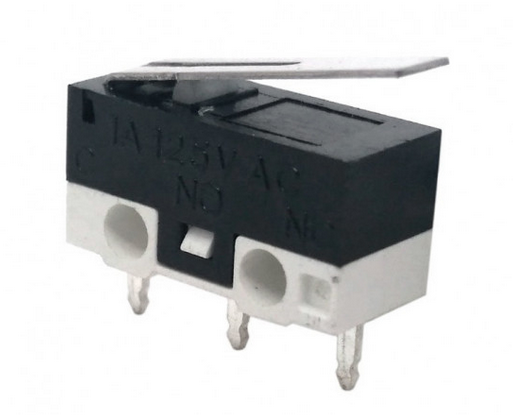
\includegraphics[width=0.2\textwidth]{figuras/eletronica/fotos_componentes/microswitch.png}\label{fig:micro_switch_pic}}
        \hspace{0.1\textwidth}
        \subfloat[][Conexões da Chave]{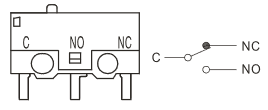
\includegraphics[width=0.3\textwidth]{figuras/eletronica/esquematicos/SW_1.png}\label{fig:micro_switch_esq}}
        \caption{Chave tipo \textit{Micro Switch}}\label{fig:micro_switch}
    \end{figure}

	\begin{itemize}
		\item[ ]
		\begin{itemize}
			\item \textbf{Alimentação:} 5 V;
			\item \textbf{Consumo de corrente máxima:} 1 A;
			\item \textbf{Quantidade de terminais:} 3;
			\item \textbf{Preço:} R\$ 0,76.
		\end{itemize}
	\end{itemize}

\subsection{\textit{Drivers} de Atuadores}
    
    Os \textit{drivers} dos atuadores são módulos projetados para prover a potência de atuação e a interação com o controle de forma simplificada. Eles convertem comandos por meio de portas lógicas em potência controlada para os atuadores. Dessa forma, tornam possível o controle automático de ações de movimento.
    
    Os atuadores que são controlados são: motor DC, atuador linear, motores de passo, solenóides para os contêineres e as mini-travas elétricas solenóides em cada compartimento de acesso no dispositivo.
    
    \subparagraph*{$\bullet$ \textbf{Motores de Passo}}\label{sec:eletronica_drivers_passo}
    
    O \textit{driver} escolhido para os motores de passo é o módulo com C.I. \textbf{A4988}, pois atende as características de carga para funcionamento do motor de passo escolhido, a partir da explicação na seção \ref{sec:energia_motor_passo} da solução energética. Além do mais, o \textit{driver} inclui a possibilidade de resolução do passo do motor em até 1/16 do considerado passo completo, assim o passo completo é o angulo mínimo, em graus, que o motor de passo realiza e é diferente para cada motor. No caso do motor escolhido, o passo completo segundo o fabricante é de 1,8$^\circ$. Por não ser uma aplicação que necessite de alta resolução para controle dos motores de passo, por apenas girar os fusos que rotacionam as engrenagens de um grupo de 5 contêineres até ser detectado a queda de um medicamento, a resolução de 1/16 do passo completo do motor é suficiente para controle.
    
    Para conexão entre o módulo de controle, especificamente o microcontrolador, e o \textit{driver} A4988 são utilizados 9 pinos, dos quais:
    
    \begin{itemize}
        \item[ ]
        \begin{itemize}
            \item[ ]
            \begin{itemize}
                \item[$\bullet$] \textbf{VCC} e \textbf{GND}: Alimentação da parte lógica.
                \item[$\bullet$] \textbf{MS1}, \textbf{MS2} e \textbf{MS3}: Portas lógicas que determinam a resolução do Passo: Passo Completo (estado lógico: ``000''); Meio Passo (estado lógico: ``100''); 1/4 Passo (estado lógico: ``010''); 1/8 Passo (estado lógico: ``001'');  1/16 Passo (estado lógico: ``111'').
                \item[$\bullet$] \textbf{\textit{ENABLE}}: Ativa (estado lógico: `1') ou desativa (estado lógico: `0') as saídas de tensão  e corrente para o motor de passo.
                \item[$\bullet$] \textbf{\textit{DIR}}: Determina a direção de rotação do motor.
                \item[$\bullet$] \textbf{\textit{STEP}}: Entrada de controle principal que cada transição de `0' para `1' realiza o movimento conforme a resolução determinada pelas portas MSx.
                \item[$\bullet$] \textbf{$\overline{\textbf{RESET}}$}:Quando vai para o estado lógico `0' ele reinicia o tradutor (bloco interno do C.I. que traduz as entradas de controle em tensões na saída para movimento do motor de passo) para um estado inicial pré-determinado e desativa todas as portas de saída para os motores. O \textit{driver} ignora todas as portas de entrada \textit{STEP} até ele voltar para o estado lógico `1' (desativado).
            \end{itemize}
        \end{itemize}
    \end{itemize}
    
    \subparagraph*{$\bullet$ \textbf{Motor DC}}
    
    O \textit{driver} escolhido para o motor DC é o \textbf{L298N}, e seu controle é baseado na ponte H. Ele atende as especificações elétricas para alimentação do motor DC escolhido, explicado na seção \ref{energ:motor_dc} da solução energética. 
    
    A estrutura de ponte H de eletrônica de potência permite a manipulação da tensão da fonte no motor por meio de chaveamento. Dessa forma, é possível controlar a velocidade do motor. Para o chaveamento, será utilizado o controle por modulação de pulso (\textit{PWM}), implementado na rotina do \textit{firmware} do microcontrolador. Essa tecnologia varia o tempo de permanência do sinal lógico em baixo e alto, acarretando em uma resposta que simula uma variação de intensidade de tensão, porém variando apenas o tempo que o sinal está ligado.  
    
    Para conexão entre o módulo de controle, especificamente o microcontrolador, e a ponte H L298 são utilizados 3 pinos:
    
    \begin{itemize}
        \item[ ]
        \begin{itemize}
            \item[ ]
            \begin{itemize}
                \item[$\bullet$] \textbf{IN1} e \textbf{IN2} (Entrada 1 e Entrada 2) são as entradas de controle do motor na ponte H. São 4 possibilidades lógicas para esses pinos: ``00'' motor gira no sentido direto, ``01'' motor gira no sentido reverso, ``10'' freio do sentido direto e ``01'' freio do sentido reverso.
                \item[$\bullet$] \textbf{GND} para conectar as referências lógicas do microcontrolador e da ponte H.
            \end{itemize}
        \end{itemize}
    \end{itemize}
    
    
    \subparagraph*{$\bullet$ \textbf{Solenoides e Atuador Linear}}
    
    O \textit{driver} escolhido para os solenoides e atuador linear foi o módulo com C.I. \textbf{IRF520N}, uma vez que atende as características elétricas requisitadas, explicado nas seções \ref{energ:solenoide} e \ref{energ:atuador_linear} da solução energética. Suas configurações possibilitam a utilização de sinais lógicos pelo microcontrolador para controle.
    
    Para conexão entre o módulo de controle, especificamente o microcontrolador, e o \textit{driver} IRF520N são utilizados 2 pinos:
    
    \begin{itemize}
        \item[]
        \begin{itemize}
            \item[]
            \begin{itemize}
                \item[$\bullet$] \textbf{SIGNAL} para o sinal lógico de controle por nível lógico.
                \item[$\bullet$] \textbf{GND} para referência da parte lógica.
            \end{itemize}
        \end{itemize}
    \end{itemize}
    

\section{Arquitetura de integração entre os módulos}\label{sec:arq_eletronica}

Nesta seção será apresentado a integração entre os módulos do sistema eletrônico. Dessa forma, são apresentados os seguintes tópicos: Conexão entre os módulos, o detalhamento dos protocolos de comunicação utilizados, a lógica de controle usando a Rede de Petri e a implementação do código-fonte para o sistema embarcado (baixo e alto nível).

\subsection{Conexão entre os Módulos}

A integração entre os módulos de medição e identificação, o de controle e o de visualização segue o diagrama de blocos da Fig. \ref{fig:fluxograma_eletronica}. Nesse diagrama é também apresentada a alimentação necessária para cada componente, explicação técnica na solução de energia no capítulo \ref{Solução_energia}.

\begin{figure}[!htb]
    \centering
    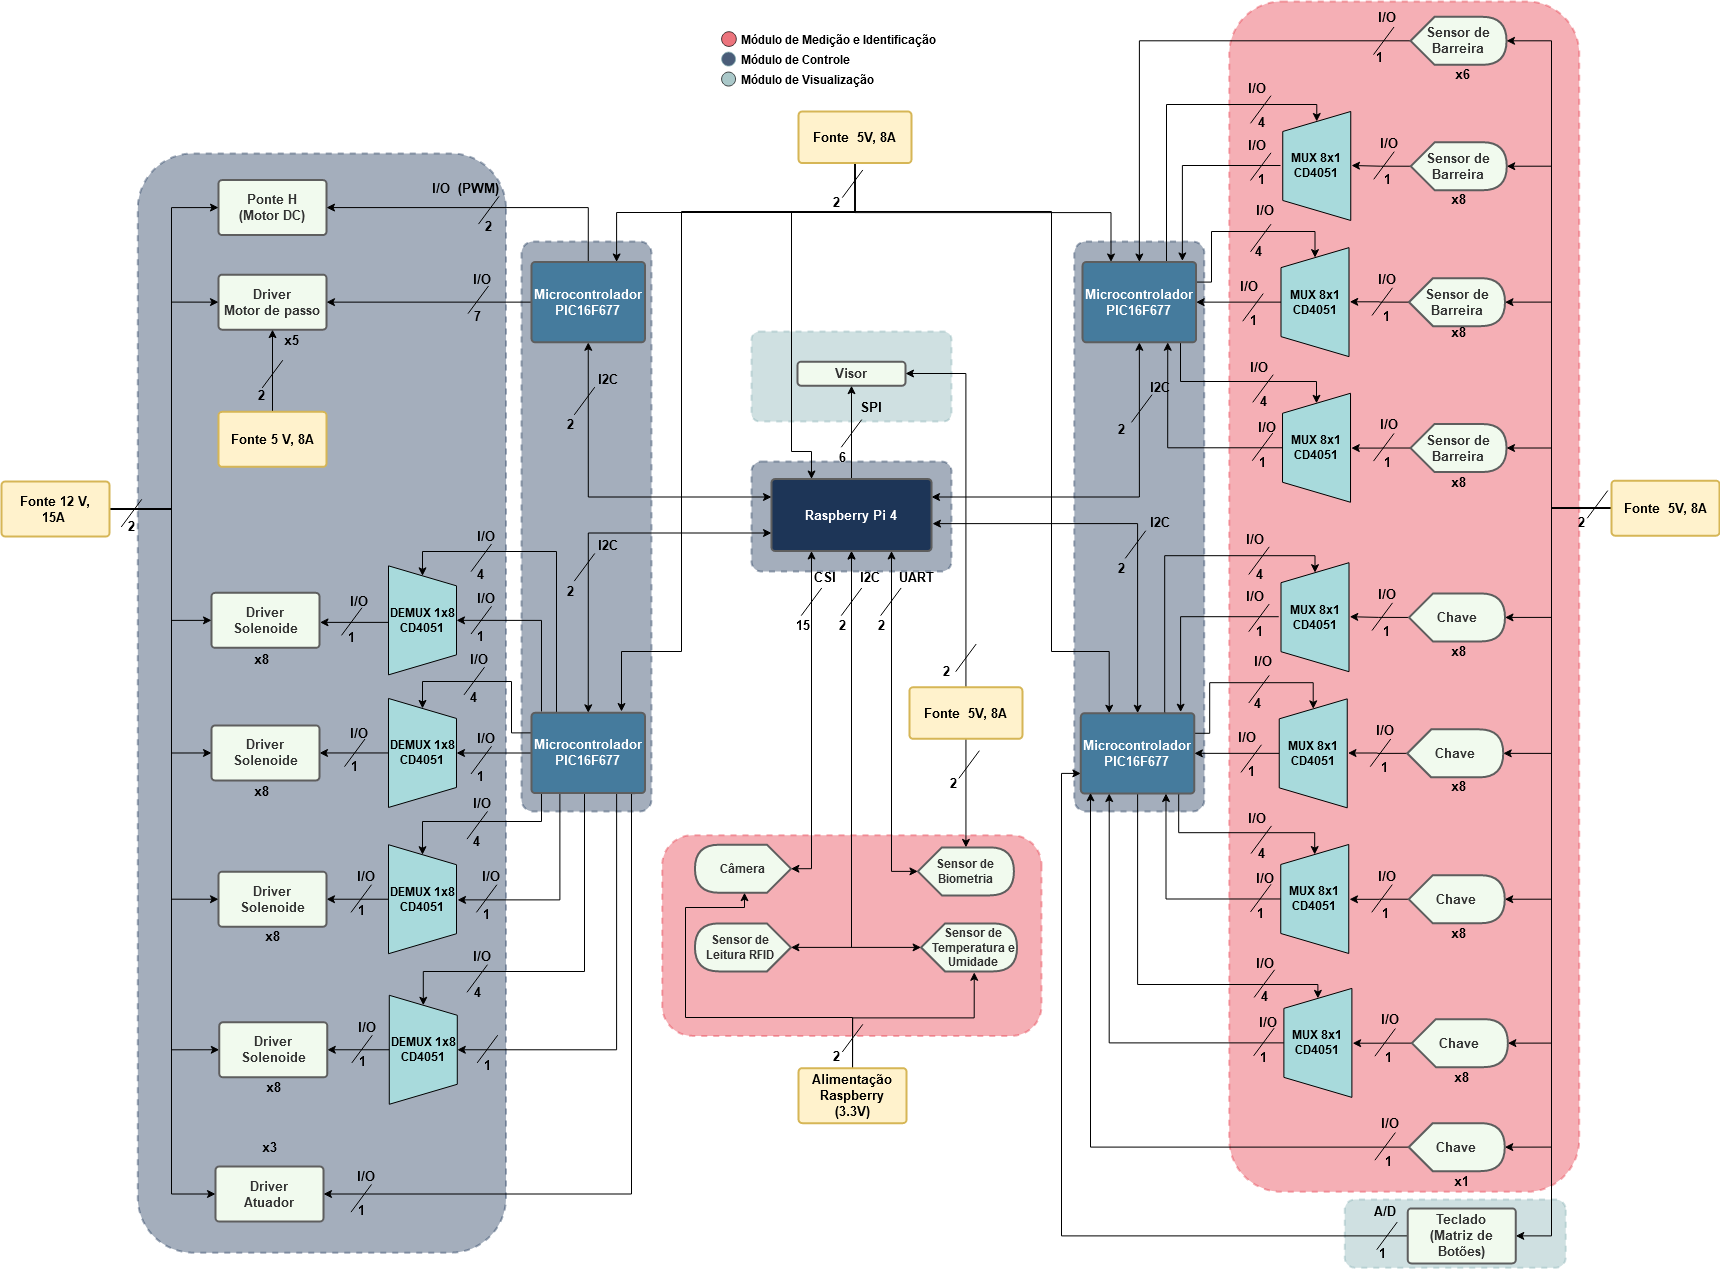
\includegraphics[width=1.1\textwidth]{figuras/eletronica/fluxogramas/fluxograma_eletronica.png}
    \caption{Diagrama Lógico Eletrônico}
    \label{fig:fluxograma_eletronica}
\end{figure}

Os diagramas esquemáticos que apresentam em detalhes as conexões entre os módulos do sistema eletrônico e respectivos componentes se encontram no apêndice \ref{esquematicos_eletronica}.

\subsection{Protocolos de Comunicação}

Os protocolos de comunicação utilizados são divididos em duas categorias: 

\begin{itemize}
    \item[$-$] \textbf{Protocolos Internos:} Utilizados para comunicação entre os módulos e respectivos componentes. São esses: I$^2$C, SPI, UART e CSI.
    
    \item[$-$] \textbf{Protocolos Externos:} Utilizados para comunicação entre o sistema eletrônico com o \textit{back-end} da solução de software. São esses: HTTP e MQTT. Esses protocolos são explicados na seção \ref{app_dispositivo}, dentro do capítulo de integração geral do dispositivo.
\end{itemize}

\paragraph*{$\bullet$ \textbf{Protocolos internos}}

\begin{itemize}
    \item I$^2$C
    
    O protocolo I$^2$C descreve o funcionamento de um barramento serial que opera com dois fios: o SCL, que é responsável por levar o \textit{clock} do dispositivo mestre para os dispositivos escravos, e o SDA, para a transferência de dados. Assim, para iniciar uma comunicação com escravos, o mestre coloca o valor lógico da linha SDA em baixo e logo em seguida é enviado o endereço do escravo que será utilizado. 
    
    Se o dispositivo escravo existir naquele endereço, um sinal de nível baixo é enviado pelo canal SCL após o oitavo pulso de \textit{clock}. Após isso, o mestre lê ou escreve nos registradores selecionados do escravo. Logo, é uma comunicação bidirecional. 
    
    Na aplicação proposta, este protocolo é usado para comunicação do dispositivo mestre, \textit{Raspberry Pi} 4, com dispositivos escravos. Os escravos são os quatro microcontroladores PIC16F677, o sensor de temperatura/umidade e o sensor RFID.
    
    \begin{figure}[H]
    \centering
    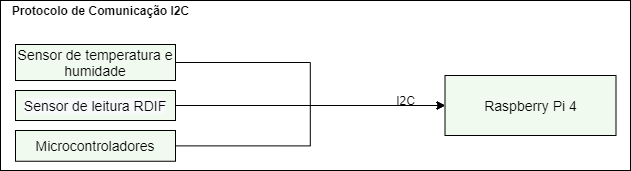
\includegraphics[width=0.7\textwidth]{figuras/eletronica/fluxogramas/comunicacao_i2c.png}
    \caption{Comunicação I$^2$C}
    \label{fig:PC_i2c}
\end{figure}
    
    \item SPI
    
    O protocolo SPI possui três fios fixos e um adicional para cada escravo no sistema. Sua comunicação é unidirecional em cada fio de comunicação, sendo o MOSI (\textit{Master Output Slave Input}) partindo do mestre para o escravo, o MISO (\textit{Master Input Slave Output}) partindo do escravo para o mestre, e o SCLK que é o \textit{clock} serial do mestre. Pa
    
    ra controlar qual escravo está sendo usado, é empregado o pino de seleção de escravo SS, que precisa de um nível baixo para operar. Por mais que este protocolo precise de mais canais para seu funcionamento, as velocidades alcançadas  superam as do I$^2$C, pois a deformação do sinal é menor pelo uso de transistores, definindo o estado do pino (Push-Pull) ao invés de dreno aberto (Pull-Up).
    
    O protocolo SPI é utilizado para comunicar o dispositivo mestre, \textit{Raspberry Pi} 4, com o visor LCD TFT 240x320, devido a ser o protocolo compatível com o controlador do visor escolhido.
    
\begin{figure}[H]
    \centering
    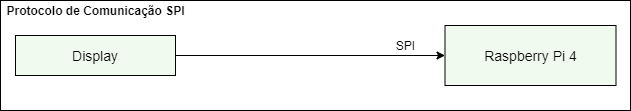
\includegraphics[width=0.7\textwidth]{figuras/eletronica/fluxogramas/comunicacao_spi.png}
    \caption{Comunicação SPI}
    \label{fig:PC_SPI}
\end{figure}

    \item UART
    
    O protocolo UART utiliza dois canais de comunicação, o RX para receber os dados e o TX para enviar. Esse protocolo trabalha de forma assíncrona, necessitando que o transmissor e o receptor estejam numa mesma taxa de transmissão (em inglês \textit{baudrate}).
    
    As conexões são feitas invertendo-se os canais em dois dispositivos distintos, ou seja, o canal TX é conectado no RX e vice-versa. Para iniciar uma transmissão, é enviado um bit de início, seguido de cinco a nove bits de informação, um bit de paridade e um a dois bits de finalização de transmissão.
    
    Este protocolo é usado para comunicar o dispositivo mestre, o \textit{Raspberry Pi} 4, com o sensor de biometria DY50.
    
\begin{figure}[H]
    \centering
    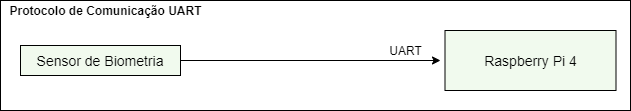
\includegraphics[width=0.7\textwidth]{figuras/eletronica/fluxogramas/comunicacao_uart.png}
    \caption{Comunicação UART}
    \label{fig:PC_UART}
\end{figure}
    
    \item CSI
    
    O protocolo CSI (\textit{Camera Serial Interface}) é caracterizado por uma fusão entre os protocolos I$^2$C e SPI. Ele utiliza duas interfaces: a primeira com os canais SCL e SDA para controle da câmera; e a segunda com um canal de transmissão unidirecional da câmera para o processador e um canal de \textit{clock} da câmera para o processador.
    
    Este protocolo é o utilizado para comunicação entre a \textit{Raspberry Pi} 4 e o módulo com câmera OV5647.
    
\begin{figure}[H]
    \centering
    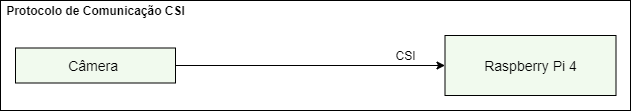
\includegraphics[width=0.7\textwidth]{figuras/eletronica/fluxogramas/comunicacao_csi.png}
    \caption{Comunicação CSI}
    \label{fig:PC_CSI}
\end{figure}
    
\end{itemize}

\subsection{Controle do Dispositivo}\label{sec:rede_petri}

A Rede de Petri é uma técnica de modelagem, a qual permite a representação de sistemas com embasamento matemático, e assim relacionar causa e efeito entre os eventos e as condições. Os elementos básicos que formam a topologia da redes de Petri são:

\begin{itemize}
    \item \textbf{Estados:} são usados para modelar os componentes passivos dos sistemas, correspondendo às variáveis de estado. No diagrama, são representadas por círculos.
    \item \textbf{Ações:} são usadas para modelar os componentes ativos dos sistemas, 
    os eventos de transição de um estado para outro. No diagrama, são representadas por retângulos.
    \item \textbf{Fluxo:} através das ações do sistema, é especificado como a transformação de um estado para outro. No diagrama, são representados por setas.
\end{itemize}

A partir do fluxograma de operação do sistema mecânico na Fig. \ref{fig:FEst}, representado na solução de estrutura na seção \ref{sec:dinamica_operacao}, elabora-se a Rede de Petri para representar e modelar o controle do dispositivo. 

Antes de iniciar o processo de controle, os medicamentos são retirados das embalagens e posicionados nos contêineres. Além do mais, os copos esterilizados também são dispostos no local de armazenamento dentro do dispositivo. A partir da Rede de Petri, na Fig. \ref{fig:rede_petri},  percebe-se que ocorrem dois processos em paralelo, a separação do medicamento e o posicionamento do copo na esteira. 

O primeiro processo tem início com o medicamento sólido no contêiner, o qual cai na comporta com a ativação do \textit{driver} do motor de passo. O medicamento é detectado pelo sensor fotoelétrico de barreira e, em seguida, deve-se desativar o \textit{drive} do motor de passo quando ocorrer a detecção, para que não caia mais de um medicamento na comporta. Posteriormente, o solenoide é ativado para abrir a comporta. Quando a comporta é aberta, o medicamento se desloca pelo canal de distribuição e, consequentemente, o solenoide é desativado. Em seguida, logo no final do funil do canal de distribuição, existe um sensor fotoelétrico de barreira para detectar a passagem do medicamento. Entretanto, quando o medicamento não é detectado pelo sensor, tem-se um aviso no visor do dispositivo que o medicamento está preso no dispositivo.

Enquanto isso, o outro processo em paralelo tem início com o copo no local de armazenamento. Sendo assim, está posicionado, no final do reservatório de copos, um sensor de barreira, para verificar e detectar a passagem do copo. Logo, quando o copo é detectado, deve-se ativar o \textit{driver} do atuador. Com a ativação do atuador, o copo é empurrado para a esteira e o \textit{driver} do atuador é desativado. Quando o copo está na esteira, é realizada a leitura da etiqueta RFID e os medicamentos são dispostos no copo a partir do posicionamento do copo abaixo do funil. Dessa forma, em uma dose medicamentosa que envolva mais de um comprimido, o copo fica esperando até atingir o final do processo de separação dos medicamentos.

Posteriormente, quando ocorre a queda de todos os medicamentos da dose individual do paciente, o \textit{driver} do motor DC na esteira é ativado e ele a rotaciona para o sentido horário. Sendo assim, quando o copo com os medicamentos é detectado por outro sensor fotoelétrico de barreira, o qual é posicionado logo abaixo da câmera, o \textit{driver} do motor DC da esteira é desativado e a esteira para, com a finalidade de realizar o captura das imagens para o processamento de imagem. 

Quando o processamento de imagens da dose individual conclui que existem erros de quantidade ou seleção, a esteira é ativada com o movimento anti-horário, até chegar em outro sensor de barreira. Esse sensor detecta que o copo com medicamento caiu no compartimento de doses medicamentosas erradas, a Zona de Retorno. Caso contrário, quando a quantidade e a seleção de medicamentos estão corretas, a esteira é ativada com o movimento horário até chegar sensor de barreira que detecta que o copo está na Área de Espera, e que o medicamento foi retirado do dispositivo. 

Portanto, quando existe um horário que mais de um paciente necessita da administração da medicação, a dose de medicamentos individuais é realizada sequencialmente para cada paciente. Quando é detectado que o copo está na zona de entrega, o dispositivo retorna para a posição inicial para a nova sequência de dose individual.

No processo de reabastecimento, em que é necessário abrir a comporta superior para adição de medicamentos e retirar os contêineres para limpeza, utiliza-se uma chave. Com ela, é possível detectar se a porta está fechada e se os contêineres estão corretamente encaixados. Caso contrário, deve-se enviar um aviso no visor para que o enfermeiro possa corrigir essas anomalias. 

\begin{figure}[H]
    \centering
    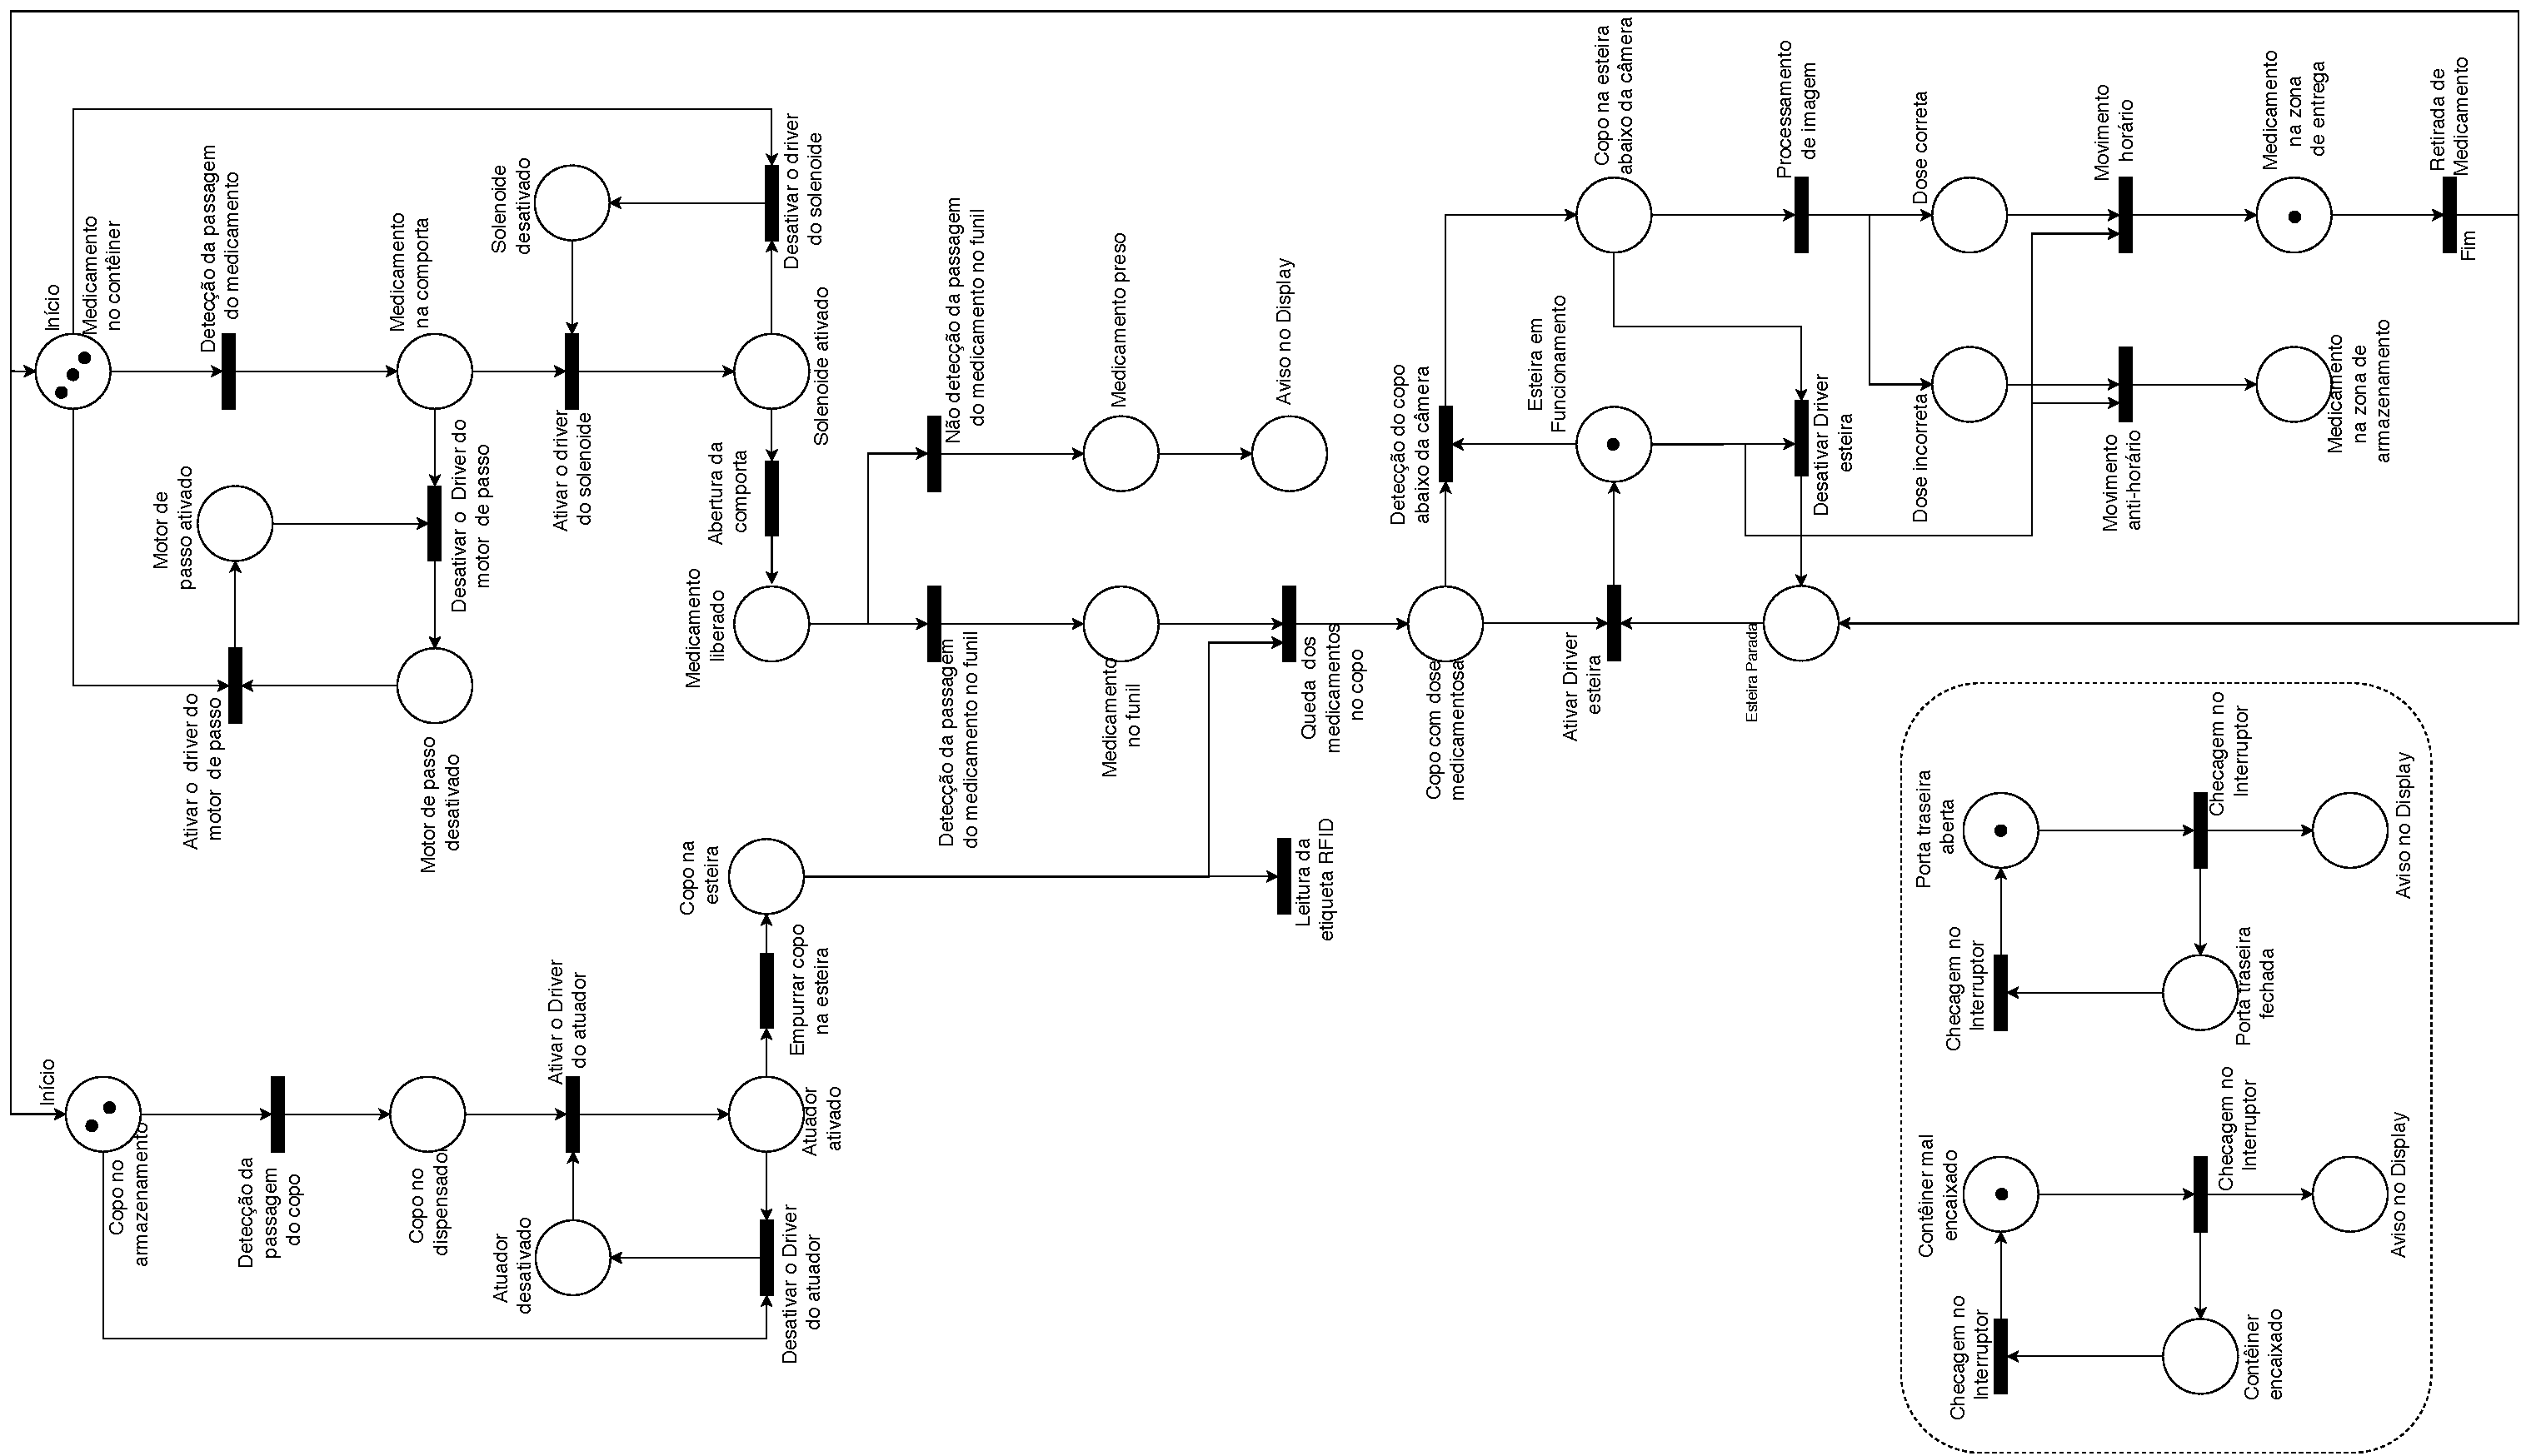
\includegraphics[width=1.4\textwidth, angle = -90]{figuras/eletronica/fluxogramas/petri.pdf}
    \caption{Rede de Petri do Controle eletrônico}
    \label{fig:rede_petri}
\end{figure}

\subsection{Código-Fonte do Sistema Eletrônico}


O código-fonte para um sistema eletrônico se refere se refere a programação de alto e baixo nível implementado para o sistema eletrônico. Sua implementação é dividida em duas partes: 

A primeira se refere aos microcontroladores da família PIC, que serão programados em baixo nível usando linguagem C por meio do compilador \textbf{CCS C}. 

A segunda se relaciona a programação em alto nível da \textit{Raspberry Pi} 4 para funcionamento do sistema eletrônico, tanto entre os módulos (medição e identificação, controle e visualização) quanto com o \textit{back-end} da solução de software. Nesse caso, a linguagem de programação utilizada é o \textit{Python 3}.

Todos os códigos desenvolvidos podem ser acessados por meio do repositório do link: \href{https://github.com/PillWatcher/pillwatcher-embarcado}{PillWatcher-Embarcado}.

\paragraph*{$\bullet$ \textbf{Microcontroladores - PIC16F677}}

O desenvolvimento de uma lógica de leitura e escrita do protocolo é necessária nos microcontroladores. O primeiro passo é ajustar o microcontrolador para o modo escravo por meio da diretiva \textbf{\#use i2c(SLAVE)}. A próxima etapa é ler o estado de comunicação por meio da função \textbf{int8 2c\_isr\_state()}. O estado retornado representa a operação que será realizada. Os estados com valores menores que \textbf{0x80} representam endereços e dados. Enquanto estados com valores iguais ou superiores a \textbf{0x80} representam a requisição de dados para o microcontrolador.

Para ler os bytes recebidos, é utilizada a função \textbf{int8 i2c\_read()}, que retorna o byte presente no \textit{buffer}. Para enviar um byte de resposta, é utilizada a função \textbf{int1 i2c\_write(unsigned int8 data)}, que escreve no barramento I$^2$C.

\paragraph*{$\bullet$ \textbf{Computador de Placa Única - \textit{Raspberry Pi} 4}}

A \textit{Raspberry Pi} 4 será programada em \textit{Python 3} por meio da utilização de bibliotecas de comunicação entre módulos do sistema eletrônico e a integração com o \textit{back-end} do software. Será descrito a comunicação e as rotinas de funcionamento do sistema eletrônico.

O processamento de imagens é implementado usando a mesma plataforma porém sua explicação é feita na seção \ref{sec:processamento_imagens}.

\subsubsection*{$-$ \textbf{Comunicação:}}

Para comunicação são determinados tanto o endereçamento específico dependendo do tipo de comunicação como os tipos de dados que são capturados ou transmitidos.

\begin{itemize}
    \item \textbf{Sensor de Temperatura e Umidade - HTU21D}
    
    Será utilizada a biblioteca \textbf{Adafruit\_HTU21D} para a comunicação com o sensor e o endereço I$^2$C empregado é \textbf{0x40}. Para capturar a temperatura e umidade será usado os métodos  \textbf{read\_temperature} e \textbf{read\_humidity} presentes na classe HTU21D.
    
    
    \item \textbf{Sensores de barreira}
    
    O código-fonte responsável pelos sensores de barreira possui em sua memória uma tabela para a seleção do sensor que será lido. Nessa tabela, estão presentes seis valores lógicos para a seleção no multiplexador, sendo três deles para seleção da porta e outros três para seleção do multiplexador ativo. O último valor na tabela se refere ao pino de entrada no microcontrolador para leitura dos sinais. Dessa forma, estão posicionados 24 sensores de barreira nos multiplexadores e 6 diretamente ligados ao microcontrolador.
    
    Para utilização do protocolo I$^2$C, foi escolhido o endereço de comunicação \textbf{0xA0}. O valor recebido representa o endereço do sensor na tabela e, dessa forma, os pinos são condicionados e o estado do sensor é enviado em retorno.
    
    \item \textbf{Sensor de Biometria - DY50}
    
    O sensor de biometria DY50 realiza todo o processamento de impressões digitais internamente em sua memória. Para enviar comandos, é utilizado o protocolo UART e, para isso, a biblioteca \textbf{python-fingerprint}. O primeiro passo é abrir comunicação serial por meio da classe \textbf{PyFingerprint}. Com ela, é possível cadastrar e identificar digitais armazenadas na memória do dispositivo.
    
    \item \textbf{Sensor RFID - PN532}
    
    Para comunicação com o sensor RFID PN532 será utilizada a biblioteca py532lib. Por meio dela, é possível ler \textit{tags} RFID utilizando os métodos na classe \textbf{Pn532\_i2c} que se comunica pelo protocolo I$^2$C. O endereço utilizado pelo sensor é o \textbf{0x24}. 
    
    \newpage
    
    \item \textbf{Câmera - OV5647}
    
    Para comunicação com a câmera, será utilizada a biblioteca \textbf{picamera}, que torna possível a aquisição de imagens por meio da classe \textbf{PiCamera} que possui o método de captura.
    
    \item \textbf{Chave e Teclado}
    
    O código-fonte segue a mesma lógica dos sensores de barreira. Contudo, possui 32 chaves conectadas em 4 multiplexadores. Dessa forma, a tabela possui 7 valores lógicos de seleção do multiplexador, com dois sensores conectados diretamente ao microcontrolador, uma chave e o teclado.
    
    Para ler os dados do teclado é utilizado o conversor A/D presente no microcontrolador, utilizando como referência a tensão de alimentação. Com isso, tem-se cinco faixas de tensão estipuladas para os parâmetros do teclado. O valor obtido da conversão é comparado com essas faixas e o botão pressionado é retornado por meio do protocolo I$^2$C com bytes com valores de 1 a 5.
    
    O endereço escolhido para comunicação I$^2$C foi \textbf{0xA2}, e os valores enviados representam o sensor requerido, com o valor 0 representado os botões e valores de 1 a 33 representando as chaves.
    
    \item \textbf{Visor - ILI9341}
    
    Para a comunicação por SPI com o visor ILI9341 será utilizada a biblioteca \textbf{Adafruit\_ILI9341}. Por meio dela, é possível desenhar formas do display e apresentar imagens utilizando a classe ILI9341.
    
    \item \textbf{Solenoides}
    
    Semelhante a como foi aplicado para os sensores de barreira, o código-fonte para as solenoides possui uma tabela com valores lógicos para seleção do requerido. Entretanto, é utilizado o modo demultiplexador, modificando o nível lógico da saída pra acionar o \textit{driver} do solenoide requerido. Os 32 solenoides são posicionados em 4 demultiplexadores, enquanto o atuador linear é conectado diretamente ao microcontrolador.
    
    Para a comunicação I$^2$C, o endereço escolhido foi \textbf{0xA4}. Os valores recebidos para o acionamento são o número do solenoide na memória e o estado de atuação ligado ou desligado, sendo que o valor 0 do endereço se refere ao atuador linear e os valores 1 a 32 representam os solenoides. O estado de acionamento é estruturado em 0 para desligado e 1 para ligado.
    
    \item \textbf{Motores de passo e DC}
    
    O código-fonte responsável pelos motores possui uma tabela com os pinos de ativação de cada motor de passo. Todos os pinos de controle dos \textit{drivers}, tanto os motores de passo quanto o motor DC, são conectados ao microcontrolador.
    
    Para a comunicação I$^2$C, o endereço escolhido foi \textbf{0xA6}. Os valores recebidos são o atuador que será acionado, 0 para o motor DC, e 1 a 5 para motores de passo. Em seguida, é recebida a direção de rotação: 0 para anti-horário, 1 para horário. Então é recebido o número de passos que o motor dará ou a ativação do motor DC. O último valor recebido representa o período dos pulsos enviados ao \textit{driver} dos motores de passo controlando a velocidade ou o \textit{Duty cycle} do PWM para o motor DC, variando de 0 a 255.
    
\end{itemize}

\subsubsection*{$-$ \textbf{Rotinas de funcionamento:}}

As rotinas de funcionamento descrevem a etapas que o sistema eletrônico realiza para executar determinada ação. Foram implementadas rotinas relacionadas ao controle do dispositivo, descritos na seção \ref{sec:rede_petri}, ao funcionamento da interface e o funcionamento de requisições vindas externamente do \textit{back-end} do software. Uma descrição mais detalhada da estrutura das requisições são descritas na seção \ref{app_dispositivo}, relacionada a integração entre o sistema eletrônico com o \textit{back-end} de software.

\begin{itemize}
    \item \textbf{Rotina de seleção de medicamento}
    
    Após receber o endereço do contêiner, a chave de encaixe correspondente é lida para checar a presença do contêiner selecionado; o motor de passo correspondente é acionado; aciona-se o solenoide correspondente e lê-se o sensor de barreira presente na saída do contêiner até a detecção da passagem do medicamento. O último passo é a detecção da passagem do medicamento pelo funil, por meio da leitura do sensor de barreira presente na saída do funil. A rotina só é acionada se houver um copo abaixo do seletor.
    
    \item \textbf{Rotina de posicionamento do copo no seletor de medicamentos}
    
    O módulo de controle aciona o atuador linear para o dispensador de copos. Em seguida, o motor da esteira é acionado e o sensor de barreira presente na posição de repouso no repositório de copos é lido até que haja detecção do copo. Feita a detecção, o motor da esteira é desligado. Em seguida, é feita a tentativa de leitura da TAG RFID presente no copo. Se a leitura for adquirida, a posição do copo é confirmada.
    
    \item \textbf{Rotina de posicionamento do copo na espera ou retorno}
    
    O módulo de controle aciona a esteira para a direção da área de espera ou da zona de retorno. O sensor de barreira respectivo é lido até a detecção da passagem do copo. Em seguida, o motor da esteira é desligado.
    
    \item \textbf{Rotina de detecção de fechamento de portas e encaixe de contêineres}
    
    Uma varredura do estado de todas as chaves de encaixe e das portas é feita a cada 15 minutos, para detectar má conexão de contêineres e/ou mal fechamento de portas.
    
    \item \textbf{Rotina de preparação de dose medicamentosa}
    
    O banco de dados de medicamentos é checado a cada 1 minuto em busca de horários de doses medicamentosas com 5 minutos adiantados. Quando há uma dose programada, as rotinas de posicionamento do copo e seleção de medicamento são feitas para cada medicamento, até completar a dose. Em seguida, é realizada a rotina de verificação dos medicamentos: Se a verificação for positiva, então o copo é posicionado na saída e a rotina de identificação de digital é iniciada.
    
    Também há a possibilidade de receber comandos para preparação dos medicamentos pelo protocolo MQTT, por meio do tópico \textit{\textbf{apply-medication}}, o que substitui a checagem do banco de dados local.
    
    \item \textbf{Rotina de biometria}
    
    A rotina espera uma impressão digital ser identificada no sensor e aciona a trava elétrica da porta especificada para abri-la. Com isso, retorna o identificador do enfermeiro e aciona a rotina de fila de doses medicamentosas, caso a porta especificada for a da área de espera.
    
    \item \textbf{Rotina de fila de doses medicamentosas}
    
    A rotina lê o sensor de barreira na porta de saída da área de espera. Quando uma dose medicamentosa é retirada e houverem mais doses preparadas na fila, a esteira é acionada 
    até a detecção do próximo copo. Consequentemente, uma mensagem de retorno é enviada ao \textit{broker} MQTT por meio do tópico \textit{\textbf{medication-response}}. O processo se repete até a fila se esgotar.
    
    \item \textbf{Rotina de atualização de dados de doses medicamentosas} 
    
    Diariamente, o módulo de controle realiza uma requisição de dados HTTP ao \textit{back-end} para obtenção de dados atualizados. Após uma conferência da integridade dos dados recebidos, o banco de dados local é trocado pelo atualizado.
    
    \item \textbf{Rotina de cadastro de enfermeiro}
    
    Por meio do protocolo MQTT, o módulo de controle escuta o tópico \textbf{\textit{create-nurse}} presente no \textit{broker} do \textit{back-end}. Quando uma nova mensagem é recebida, a máquina aciona o visor com uma mensagem para cadastro do enfermeiro recebido.
    
    Assim, o leitor de impressões digitais é acionado para cadastro. Quando a digital é cadastrada com sucesso, uma mensagem de sucesso é escrita na tela. Quando há erro no cadastro, uma mensagem de erro é escrita, e o sensor é acionado novamente para cadastro.
    
    \item \textbf{Rotina de abastecimento de medicamentos}
    
    Por meio do protocolo MQTT, são escutados os tópicos \textit{\textbf{create-medication}} e \textit{\textbf{create-supply}}. Quando há uma nova entrada, ela é adicionada ao banco de dados de medicamentos, e aciona a rotina de biometria.
    
    \item \textbf{Rotina de abastecimento de copos}
    
    Por meio do menu presente no visor, o reabastecimento de copos será requisitado e, com isso, a rotina de biometria é acionada.
    
    \item \textbf{Visor}
    
    O visor possui diferentes estados, possuindo diferentes telas de interação e um menu. Porém, para o projeto, sua implementação não foi concluída, e um modelo de alta fidelidade foi desenvolvido e se encontra no Apêndice  \ref{app_telas_display}. O princípio de funcionamento é por meio da detecção dos botões que navegarão pelos estados possíveis do visor e acionarão funções de configuração presentes no modelo.
    
\end{itemize}

\section{Processamento de Imagens}


\subsection{Separação dos comprimidos}


A primeira etapa para extrair dados da imagem é isolar os comprimidos presentes. Para isso é preciso a conversão da imagem para escala de cinza, facilitando assim na utilização de operações de filtragem na imagem em etapas subsequentes. Para exemplificar a explicação daqui em diante utilizamos uma imagem do banco de dados, original na figura \ref{fig:proOrig}, e aplicando a conversão para escala de cinza temos o resultado na figura \ref{fig:proCinza}.

Em seguida, é necessário a detecção das bordas do comprimido. Como as imagens do banco de dados possuem um fundo padronizado o uso da técnica de limiar é possível. Um resultado possível pode ser observado na figura \ref{fig:proLim}. 

O próximo passo é eliminar resíduos da imagem deixando apenas o contorno do comprimido. Para isso são realizadas operações de abertura e fechamento utilizando elementos estruturantes circulares maiores que o resíduo e menores que o comprimido. Com isso obtemos uma máscara do exemplo utilizado, na figura \ref{fig:proMask}.

Por fim, uma técnica de detecção de objetos conectados é aplicada, a qual consegue separar objetos na imagem por meio de observação da vizinhança na imagem. Aplicando essa técnica nos exemplos temos o resultado nas figuras \ref{fig:proMask1} e \ref{fig:proMask2}.

Com a máscara segmentada é possível separar os comprimidos por meio de uma multiplicação com a imagem original, com isso obtemos as figuras \ref{fig:proPill1} e \ref{fig:proPill2}.

\begin{figure}[H]
        \centering
        \subfloat[][Original]{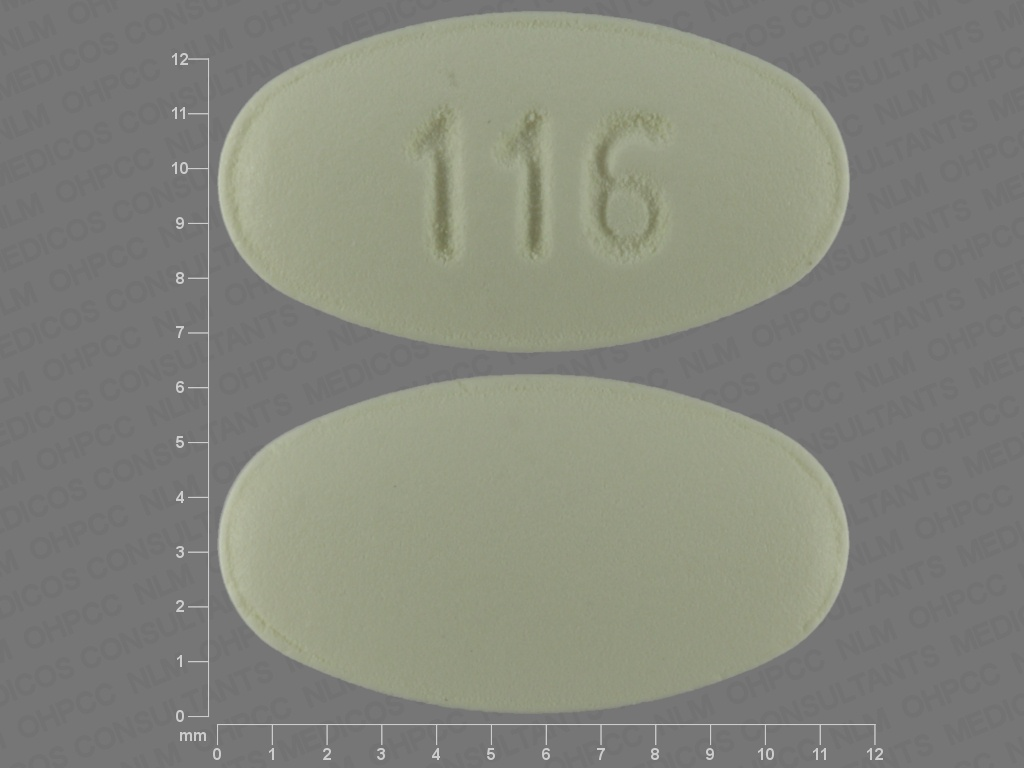
\includegraphics[width=0.3\textwidth]{figuras/processamento/original.jpg}\label{fig:proOrig}}
        %\hspace{0.1\textwidth}
        \subfloat[][Escala de cinza]{
        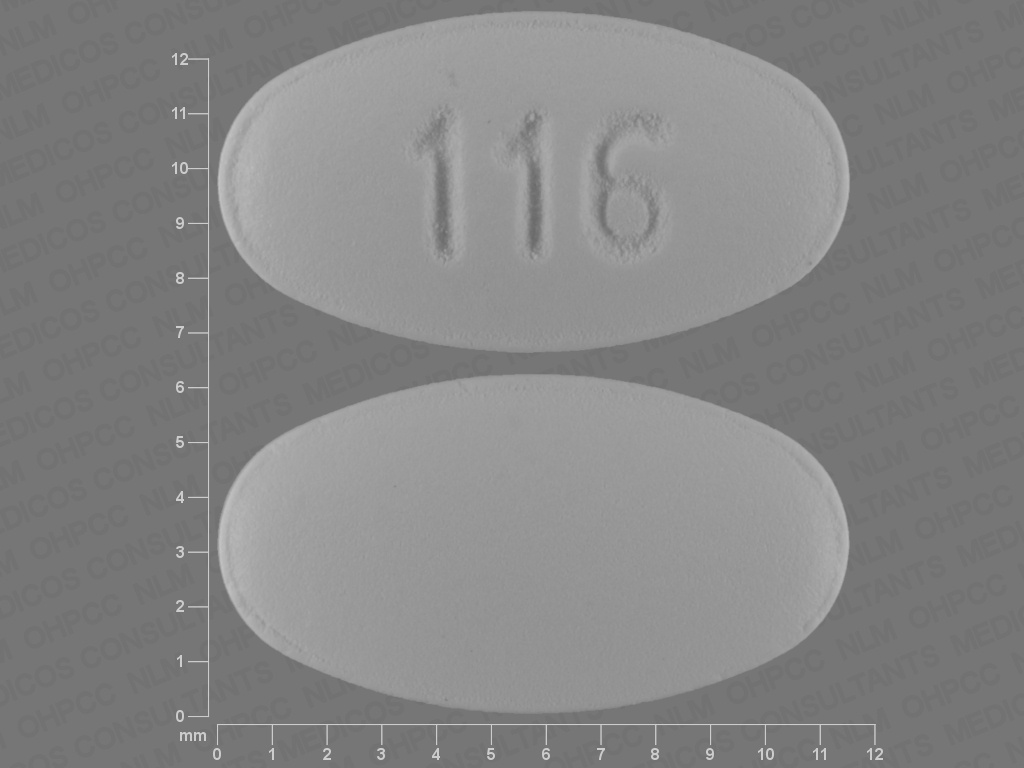
\includegraphics[width=0.3\textwidth]{figuras/processamento/cinza.jpg}\label{fig:proCinza}}
        \subfloat[][Limiar]{
        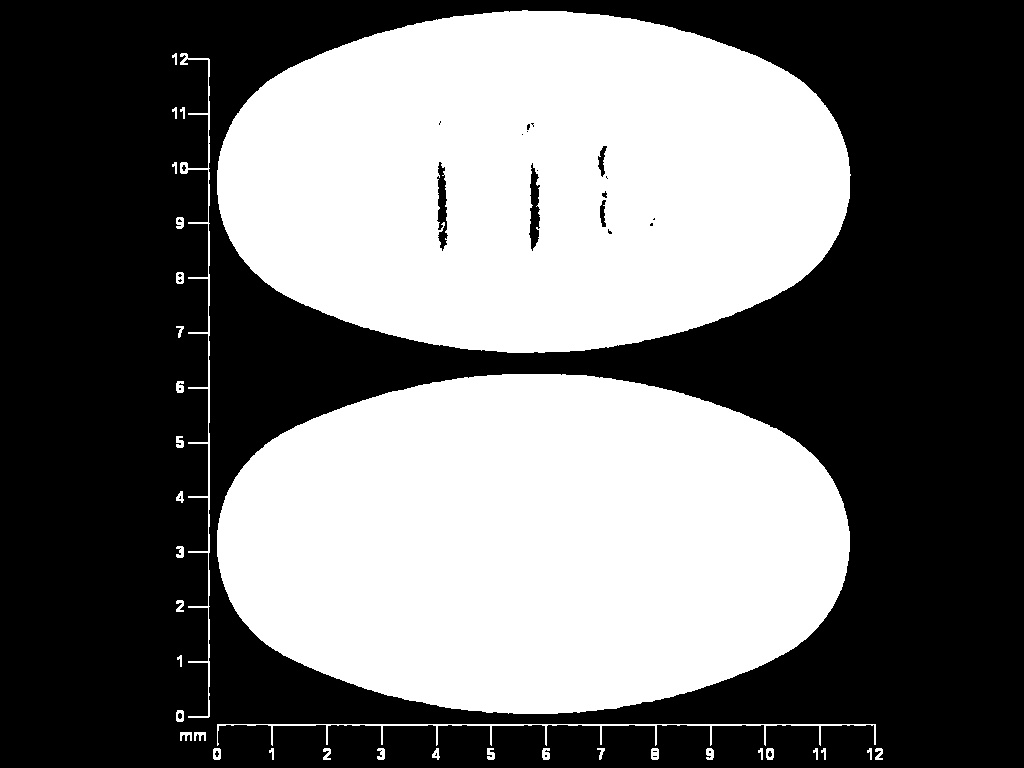
\includegraphics[width=0.3\textwidth]{figuras/processamento/limiar.jpg}\label{fig:proLim}}
        
        \subfloat[][Máscara]{
        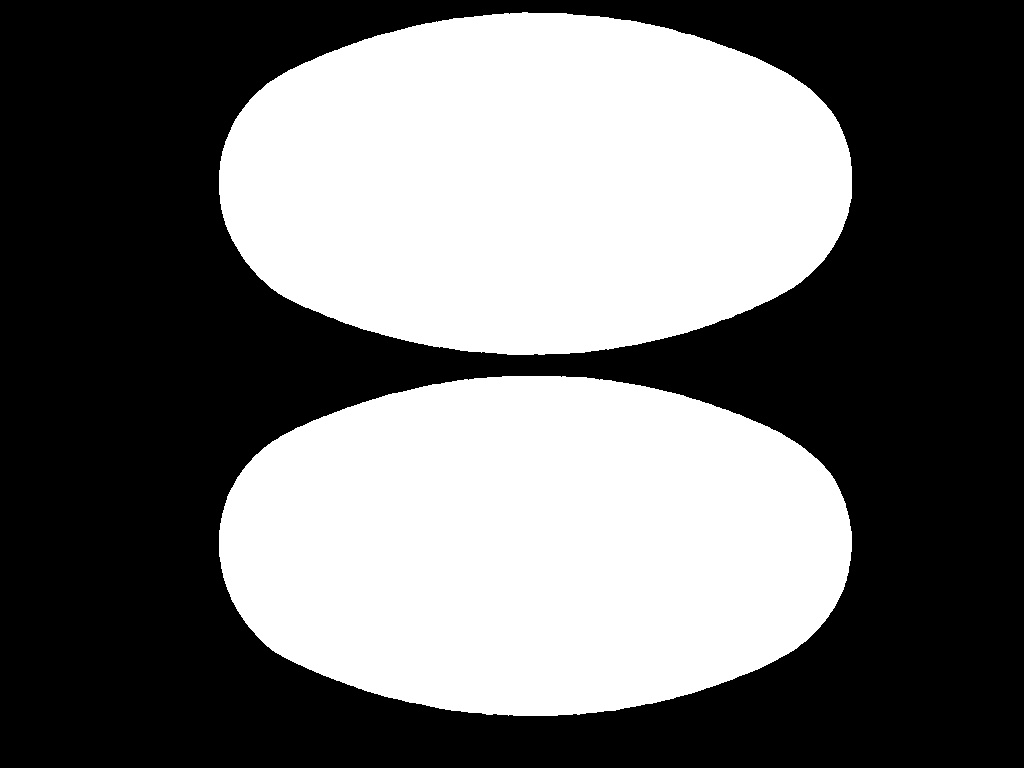
\includegraphics[width=0.3\textwidth]{figuras/processamento/mascara.jpg}\label{fig:proMask}}
        \subfloat[][Objeto 1]{
        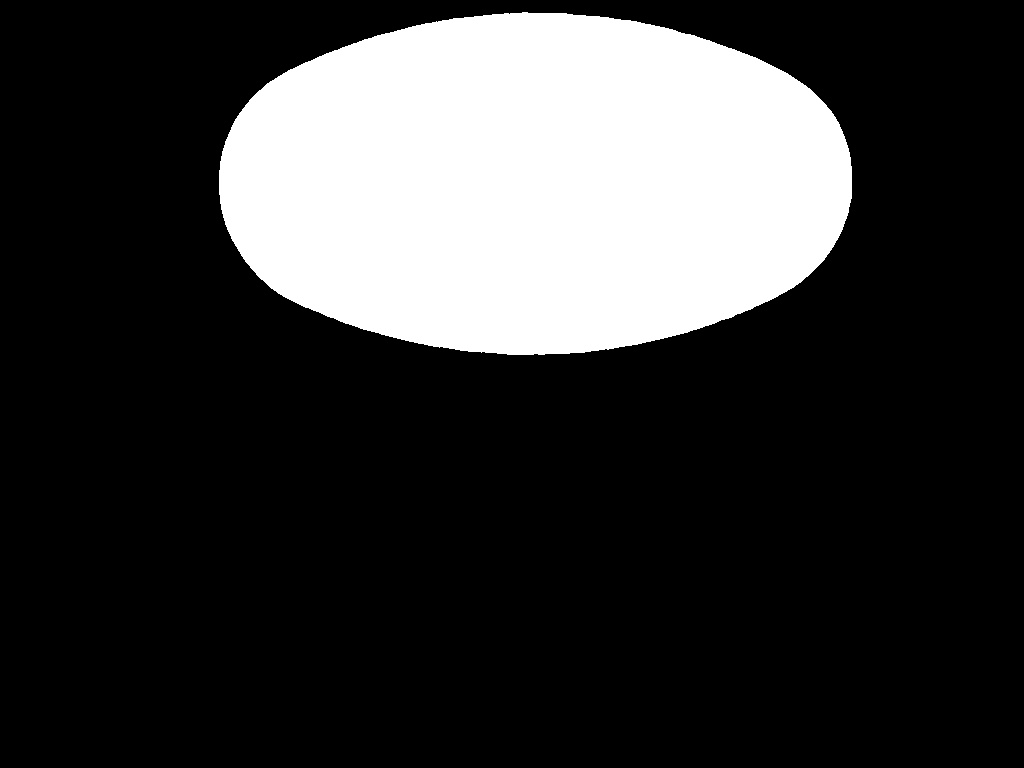
\includegraphics[width=0.3\textwidth]{figuras/processamento/mascara1.jpg}\label{fig:proMask1}}
        \subfloat[][Objeto 2]{
        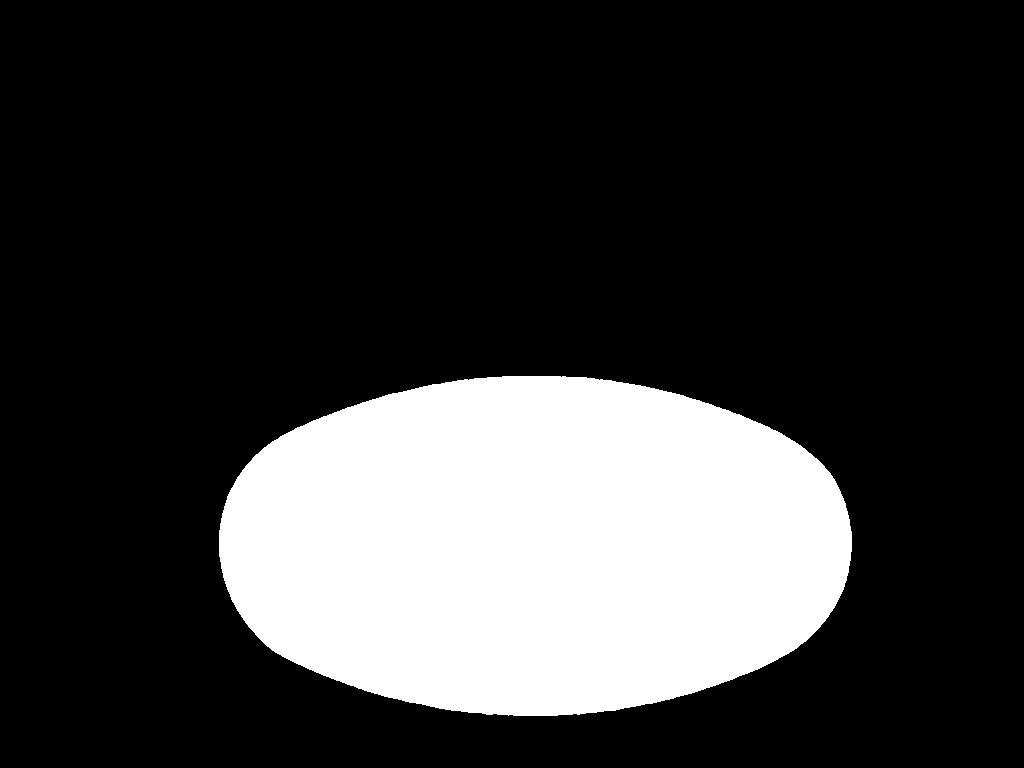
\includegraphics[width=0.3\textwidth]{figuras/processamento/mascara2.jpg}\label{fig:proMask2}}
        
        \subfloat[][Comprimido 1]{
        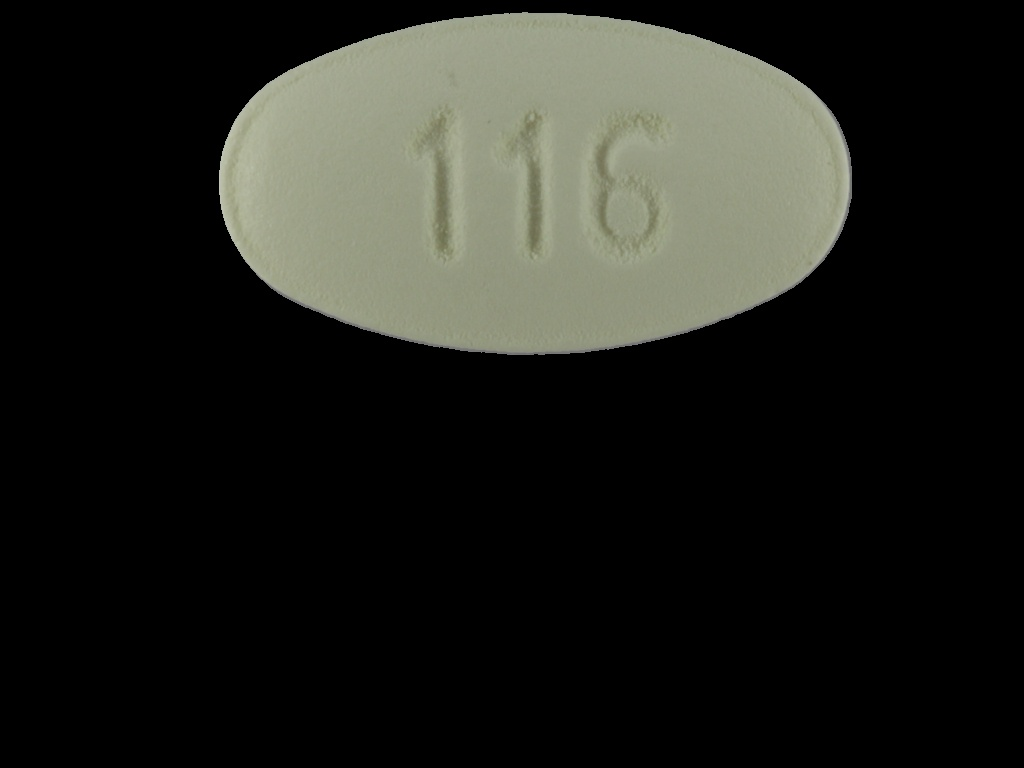
\includegraphics[width=0.3\textwidth]{figuras/processamento/pilula1.jpg}\label{fig:proPill1}}
        \subfloat[][Comprimido 2]{
        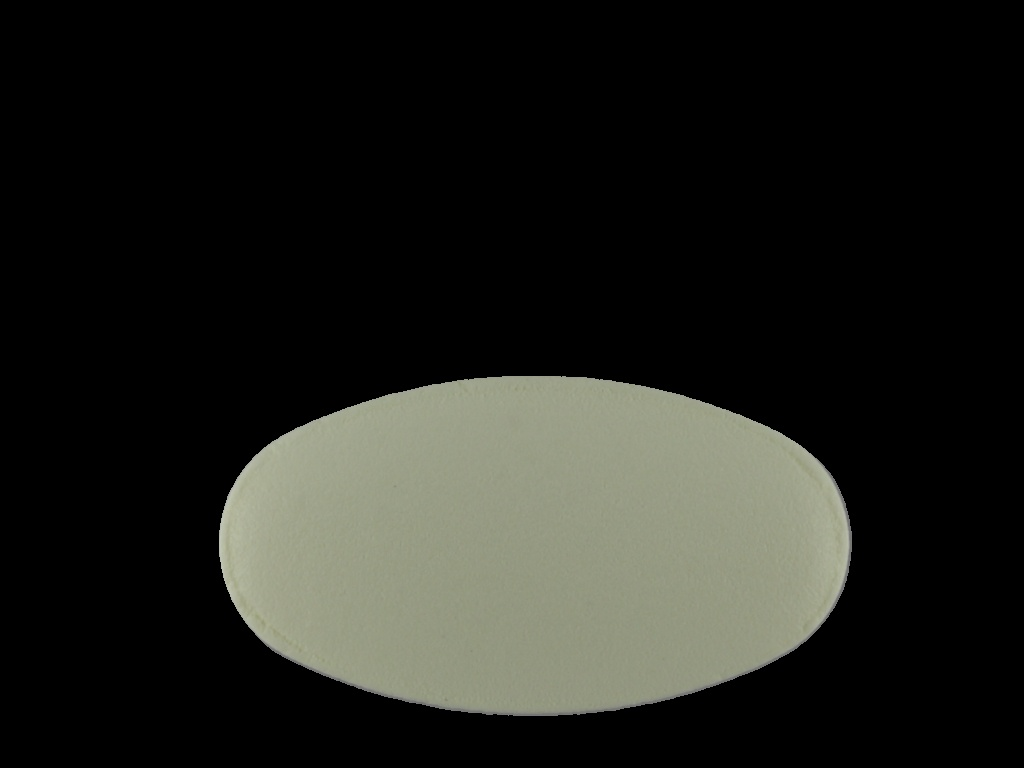
\includegraphics[width=0.3\textwidth]{figuras/processamento/pilula2.jpg}\label{fig:proPill2}}
        
        \caption{Processo de separação}
        \label{fig:proCond}
\end{figure}

\subsection{Extração de características}

Com os comprimidos separados é possível extrair informações que serão utilizadas para classificá-los.

\begin{itemize}
    \item \textbf{Cor}
    
    Para extrair a cor do comprimido será utilizada uma média de cor de toda a região, eliminando possíveis efeitos de sombra presentes. Sendo assim, serão estabelecidos rótulos que corresponderão a uma faixa específica do espectro RGB das imagens.
    
    \newpage
    \item \textbf{Formato}
    
    Para extrair o formato do comprimido será utilizada a técnica de \textit{template matching}. Ela consiste em comparar a imagem com modelos pré-definidos, realizando a correlação da imagem com o \textit{template}, Se essa correlação for próxima de 1 significa que há uma alta probabilidade do formato estar correto. Consequentemente, é possível testar todos os formatos possíveis e identificar qual a maior correlação entre eles.
    
    \item \textbf{Texto estampado}
    
    Para extrair o texto do comprimido é necessário o tratamento da imagem para que os contornos sejam destacados com isso obtemos a figura \ref{fig:propilLim}, porém o objeto de texto ainda possui áreas não conectadas. Para contornar esse problema é utilizado uma abertura na imagem com um objeto estruturante circular pequeno com até 5 pixeis de diâmetro. Assim obtemos como resultado uma melhor definição das letras, mostrado na figura \ref{fig:propilAb}.
    
    Por fim, subtrai-se a máscara do comprimido do resultado anteriormente obtido e, consequentemente, no isolamento do texto a ser processado. O resultado da subtração da máscara pode ser visualizado na figura \ref{fig:propiltext}.
    
    Para interpretar o texto será utilizado o \textbf{Tesseract}, um sistema de reconhecimento óptico de caracteres (OCR) que utiliza uma rede neural treinada para identificar linhas de texto. Para utilização desse sistema é necessário identificar a região de interesse e isolá-la para melhores resultados. Assim obtemos o resultado na figura \ref{fig:propiltextex}, onde é possível observar a região de interesse que possui texto e o valor reconhecido.
    
    \begin{figure}[H]
        \centering
        \subfloat[][Destaque dos contornos]{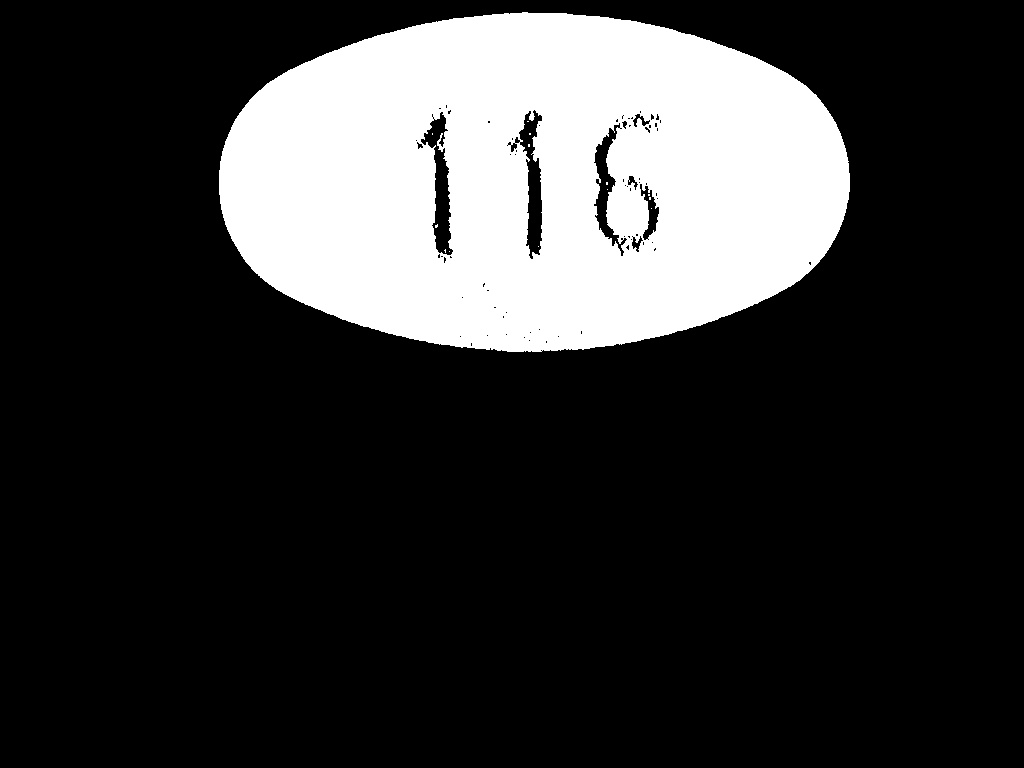
\includegraphics[width=0.3\textwidth]{figuras/processamento/pilulalimiar.jpg}\label{fig:propilLim}}
        \hspace{0.05cm}
        \subfloat[][Conexão das letras]{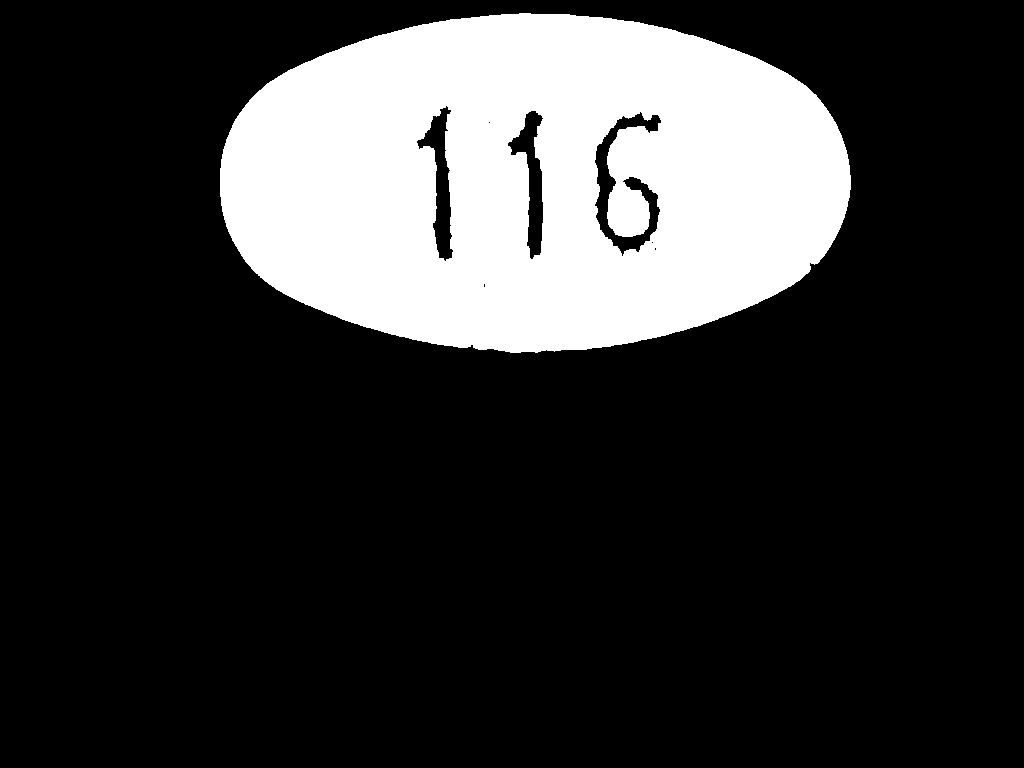
\includegraphics[width=0.3\textwidth]{figuras/processamento/pilulaabertura.jpg}\label{fig:propilAb}}
        \hspace{0.05cm}
        \subfloat[][Texto isolado]{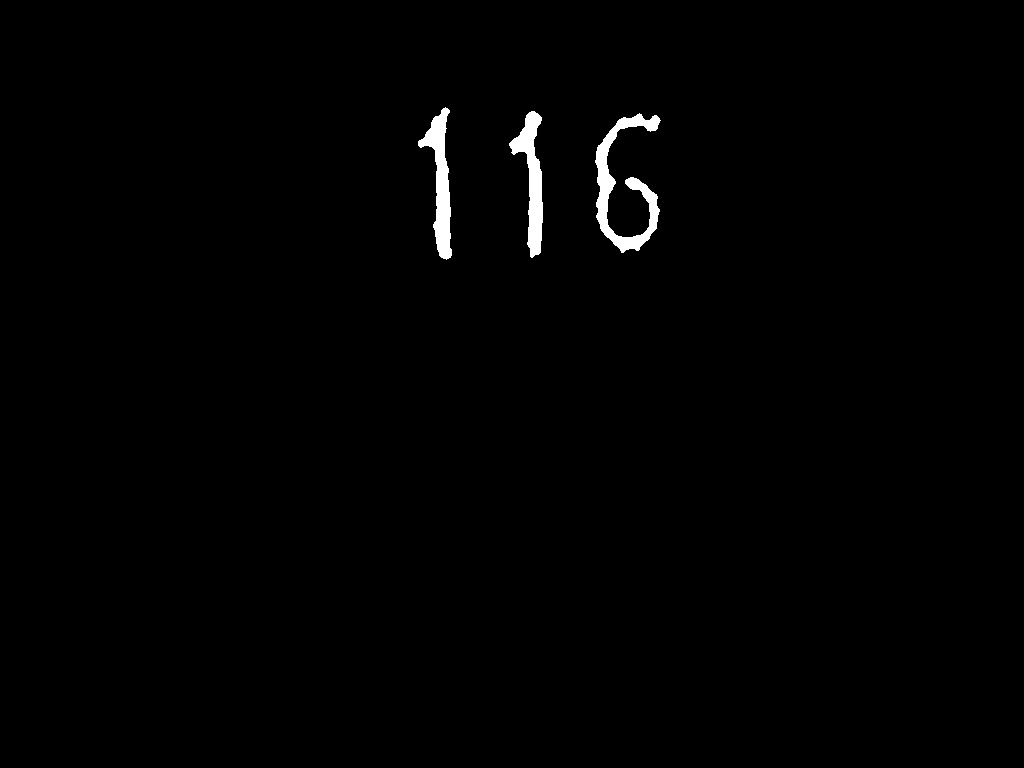
\includegraphics[width=0.3\textwidth]{figuras/processamento/texto.jpg}\label{fig:propiltext}}
        
        \subfloat[][Texto identificado]{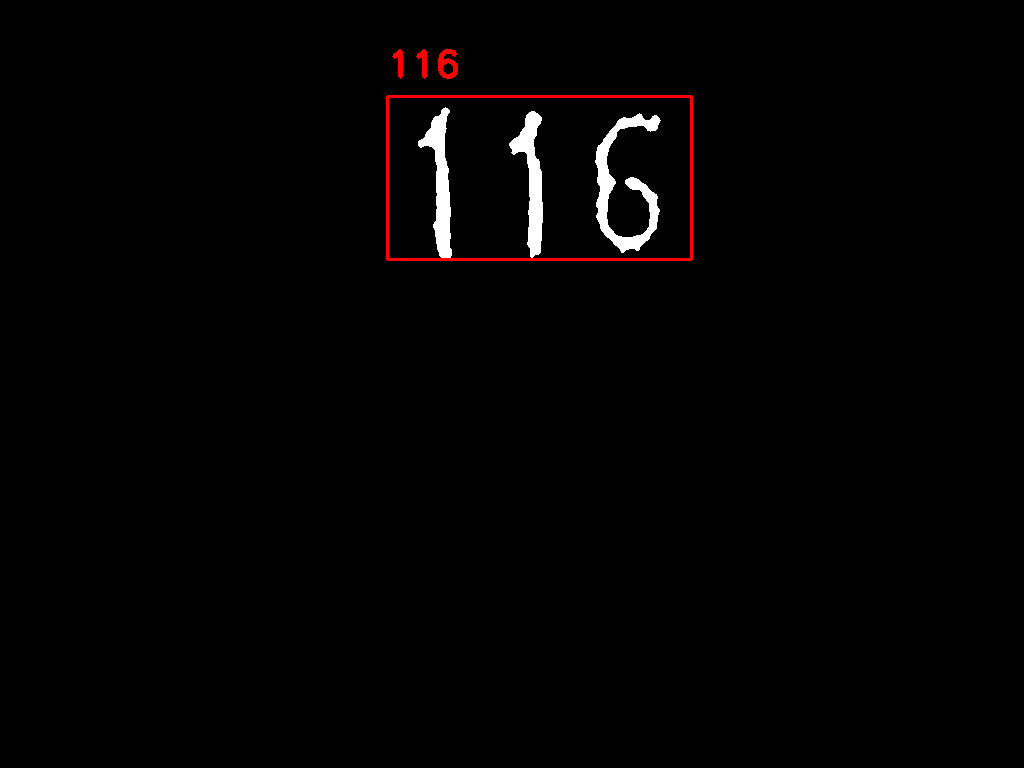
\includegraphics[width=0.4\textwidth]{figuras/processamento/textoExtraido.png}\label{fig:propiltextex}}
        
        
        \caption{Extração de texto}
        \label{fig:proText}
    \end{figure}
\end{itemize}

\subsection{Máquina de Vetores de Suporte (SVM)}

Para conseguir identificar diversos comprimidos nas imagens é necessário o uso de um classificador. Existe diversos tipos de classificos e o escolhido foi a máquina de vetores de suporte (SVM). 

Seu funcionamento se baseia na ideia de gerar uma superfície que separa as classificações por meio das características empregadas. Dessa forma são criados vetores de suporte que separam a área entre classificações, gerando assim os vetores de suporte que deve haver o treinamento da SVM.

Para o treinamento será utilizado um banco de imagens de comprimidos feito pela \textit{National Library of Medicine} que possui 4000 imagens em ambiente controlado e 133000 em imagens amadoras, disponível no  \href{https://www.nlm.nih.gov/databases/download/data_distrib_main.html}{link}. 

O tipo de classificação utilizada será a \textit{yes or no}. Na qual serão criadas SVMs para cada comprimido a ser identificado e ensinando ela para identificar características daquele comprimido.



\section{Plano de Construção}
\label{sec:plano_de_construção}

A construção dos módulos do sistema eletrônico foi implementada a partir dos esquemáticos descritos na seção \ref{sec:arq_eletronica}. Desses esquemáticos, podem ser geradas as placas de circuito impresso (PCI), que servem como base para conexão de todos os módulos e seus componentes do sistema eletrônico. 

Para o projeto das PCIs, foi utilizado o software \textit{Proteus} e tem-se o emprego de placas de fibra de vidro de camada dupla de 1,6 mm de espessura. Em algumas PCIs, a camada oposta possui vias passantes para realizar conexões. A largura mínima da trilha é determinada pela espessura do cobre da placa e a corrente máxima que percorre o circuito. Assim, a partir da seleção de uma placa com 3 onças (oz) de espessura de cobre da placa, aproximadamente 85 gramas, e uma corrente máxima de 3 A, é possível determinar a largura da trilha, utilizando as fórmulas IPC-2221. Primeiramente, deve-se calcular a área da seção transversal conforme a Eq. \ref{IPC-2221}:

\begin{equation}\label{IPC-2221}
    A = \frac{i \; [\text{A}]}{\left[ k \; [\frac{\text{W}}{\text{m} \cdot ^\circ \text{C}}] \cdot(dT \; [^\circ \text{C}]\textsuperscript{0,44})\right]^{\frac{1}{0,725}} } \quad [\text{mils}^2]
\end{equation}

Em que $A$ é a área da seção transversal, $i$ é a corrente máxima, $dT$ é o aumento da temperatura acima da temperatura ambiente e $k$ é a constante de condutividade térmica, a qual, para camadas internas, $k=0,024$, enquanto que, para camadas externas, $k=0,048$ \cite{IPC}. Em seguida, a largura é calculada conforme a Eq. \ref{IPC-2221_2}:

\begin{equation}\label{IPC-2221_2}
    L = \frac{A \; [\text{mils}^2]}{\left[(E \; [\text{oz}] \cdot 1,378 \; [\frac{\text{mils}}{\text{oz}}])\right]} \quad [\text{mils}]
\end{equation}

Em que $L$ é a largura da trilha e $E$ é a espessura do cobre na placa. Assim, a partir das Eq., determinou-se que a trilha deve possuir 17,9 mils, aproximadamente 0,456 mm. Entretanto, para o projeto das PCIs, foi adicionado uma folga na largura da trilha. Logo, foi utilizado 25 mils, correspondente a 0,635 mm.

Além do mais, as angulações para todas as PCIs foram de 45$^\circ$ e 60$^\circ$ para as vias roteadas, a distância de uma trilha para outra foi de 15 mils (0,381 mm), já que o mínimo é 9 mils (0,229 mm), a distância de uma trilha para um furo é de no mínimo 8 mils (0,200 mm) e a distância entre as inscrições da serigrafia e os \textit{pads} (\textit{SMD}, \textit{Through Hole} e BGA) seja, no mínimo, de 5 mil (0,127mm).

Ademais, foram utilizados conectores \textit{Molex} KK e uma legenda em cada conector da PCI para evitar a conexão errada de algum componente, tanto em tipo quanto na orientação do cabo. As figuras no apêndice \ref{app:PCB} mostram os \textit{layouts} para as placas fabricadas. Em todos os casos, foram utilizadas zonas preenchidas de \textit{Ground} (GND) na camada de cobre.

A descrição da conexão das PCIs e os componentes eletrônicos está detalhada no manual de montagem (seção Conexão dos Componentes eletrônicos), apêndice \ref{manual_montagem}.

\section{Plano de Testes}

Os procedimentos descritos nessa seção tem o objetivo de verificar a conformidade dos resultados entre o sistema construído e o que foi projetado, garantindo, assim, que cada componente funcione conforme foi projetado e, consequentemente, o sistema eletrônico ao integrá-los. 

\subsection{Teste do módulo de controle}\label{sec:teste_cc}

\subparagraph*{$\bullet$ Sistema Embarcado} \hfill

O teste do módulo de controle começa verificando se a cópia da imagem do software com o sistema operacional (OS) para \textit{Raspberry Pi} 4 foi bem sucedida. 

Com o OS funcionando corretamente, se da inicio ao processo de verificação da conexão entre a \textit{Raspberry Pi} 4 e os componentes conectados ao protocolos I$^2$C (quatro microcontroladores, um sensor de temperatura e umidade HTU21D e um sensor RFID PN532), UART (um sensor biometria - DY50) e CSI (uma câmera OV5647. 

Para o protocolo I$^2$C, o dispositivo mestre (\textit{Raspberry Pi} 4) requisita dos dispositivos escravos seus endereços de identificação interno, sendo isso um valor fixo armazenado no registrador de identificação interno e descrito no \textit{datasheet} para cada componente. 

Os valores hexadecimais a serem lidos são:

\begin{enumerate}
    \item[]
    \begin{itemize}
        \item Quatro microcontroladores: 0xA0, 0xA2, 0xA4 e 0xA6;
        \item Sensor RFID - PN532: 0x24
        \item Sensor temperatura e umidade - HTU21D: 0x40
    \end{itemize}
\end{enumerate}

Para UART e CSI são utilizados os programas específicos desenvolvidos com base no manual fornecido pelo fabricantes. Eles verificam e validam a conexão apropriada com o módulo de controle e o funcionamento do sensor de biometria e câmera.

\subsubsection*{$-$ Chave: Micro \textit{Switch} KW10-B:}

Para as chaves são realizados os seguintes testes:

\begin{enumerate}
    \item Teste individual de continuidade e funcionamento mecânico:
    
    \begin{itemize}
        \item \textbf{Objetivo:} Verificar se a chave tem algum defeito de fabricação e está funcionando como esperado;
        \item \textbf{Itens necessários:} Multímetro;
        \item \textbf{Procedimento:} 
        \begin{enumerate}
            \item Conectar as pontas de prova do multímetro com os terminais 1 e 2 da chave;
            \item Pressionar de forma contínua para ver a continuidade e resistência entre os terminais;
            \item Pressionar a haste de ativação da chave em várias velocidades diferentes (menor para maior), observando se aparece alguma ativação falso positiva;
        \end{enumerate}
    \end{itemize}
    
    \item Teste de detecção entre módulo de controle e chave:
    
    \begin{itemize}
        \item \textbf{Objetivo:} Verificar se o módulo de controle está conseguindo detectar a abertura e fechamento de cada chave;
        \item \textbf{Itens necessários:} \textit{Raspberry Pi} 4 rodando programa específico para esse teste;
        \item \textbf{Procedimento:} 
        \begin{enumerate}
            \item Conectar todas as chaves a respectiva PCI e ela na \textit{Raspberry Pi}, conforme descrito no manual de montagem (apêndice \ref{manual_montagem});
            \item Executar o programa de testes para as chaves. Objetivo é ver a resposta do respectivo microcontrolador associado as chaves;
            \item Pressionar cada chave individualmente para verificar se estão sendo detectadas;
            \item Pressionar todas as chaves ao mesmo tempo e solta-las. Verifica se é traduzido no módulo de controle verificar que todas estão fechadas e depois abertas.
        \end{enumerate}
    \end{itemize}
    
\end{enumerate}

\subsubsection*{$-$ Teste dos Atuadores:}

Os testes realizados para os atuadores tem o objetivo de verificar se o funcionamento dos componentes utilizados atendem a simulações de controle ou cálculos, observando por um ponto de vista da parte elétrica com enfase no controle. A explicação por um ponto de vista estritamente elétrico da alimentação dos motores, assim como de características elétricas, são descritas no plano de teste da solução de energia, seção \ref{sec:plano_teste_energia}.

Para cada atuador, são realizadas 3 fases de testes sendo: Teste Inicial, Teste Parcialmente Integrado e Teste Completamente Integrado, seguindo o seguinte procedimento:

\subparagraph*{} $*$ \textbf{Teste Inicial:}
    
Nessa fase, cada componente relacionado ao funcionamento dos atuadores é testado por um ponto de vista elétrico, como testes de comportamento elétrico ao interligar \textit{driver} e atuador, e de operação do respectivo microcontrolador que realiza a distribuição do sinal de controle com os atuadores, sendo realizado para validar a correta funcionalidade dos componentes comparado ao que era esperado.
    
\subparagraph*{} $*$ \textbf{Teste Parcialmente Integrado:} \hfill 

Nessa fase de teste, alguns componentes elétricos são interligados para mostrar que essa integração vai ter mínimo impacto no comportamento dos atuadores, sendo analisado principalmente o erro. Isso é realizado com uma integração simples do atuador e seu respectivo \textit{driver} com o módulo de controle, onde é executado vários testes simples do controle, e são realizadas medições de várias tolerâncias que impactam o projeto. Essa etapa é crucial para realizar a calibração e implementar ajustes necessários antes de fixação dos atuadores no dispositivo protótipo.
    
\subparagraph*{} $*$ \textbf{Teste Completamente Integrado:} \hfill

Nessa fase, os componentes mecânicos do dispositivo são integrados com os componentes elétricos previamente testados. Os principais pontos testados e analisados são as tolerâncias e se o funcionamento correto dos atuadores sob condições normais de carga atendem e superam as especificações projetadas. 

\subparagraph*{$\bullet$ \textit{Driver} Motor de Passo: A4988} \hfill

\subparagraph*{} $-$ Teste inicial:\label{sec:teste_inicial}

O primeiro teste consiste em realizar medições da tensão elétrica de alimentação e sinal de controle entre motor de passo, \textit{driver} e circuito integrado com microcontrolador.  O equipamento necessário para essa medição é um multímetro. Nesse teste, temos o seguinte critério a se satisfazer:


\begin{itemize}
    \item[$\bullet$] $V_\text{alimentação}$ = 12 V
    \item[$\bullet$] $V_\text{controle}$ = 5 V 
\end{itemize}

O procedimento consiste em testar cada terminal e GND para verificar se a tensão fornecida pela fonte de alimentação para o \textit{driver} A4988 está correta, se repetindo para os 5 utilizados.

Completando o primeiro teste, é garantido que os componentes usados atendem as especificações técnicas elétricas e não estão com defeito, assim como as perdas no cabo não são bem especificadas.

O segundo teste é para testar a operação do circuito integrado com microcontrolador, sendo verificado a resposta dos vários sinais de controle do \textit{driver} para uma rotina normal de operação. As especificações analisadas são as seguintes:

\begin{enumerate}
    \item Geração do sinal lógico para entrada \textit{STEP}
    \item Nível lógico para as outras 6 entradas (MS1, MS2, MS3, DIR, ENABLE, RESET).
    \item Modos de operação:
    \begin{enumerate}
        \item Modo de espera;
        \item Operação na velocidade máxima;
        \item Operação na metade da velocidade;
        \item Operação de parada;
        \item Modo de inicialização;
        \item Cenário com falha na alimentação.
    \end{enumerate}
\end{enumerate}

No procedimento de teste, é utilizado um programa básico rodando na Raspberry Pi 4, que simula o controle dos motores de passo. Para medição dos terminais, é utilizado o osciloscópio, para verificar se os sinais gerados estão condizentes com o desenvolvido para o projeto. 

O critério para aprovação é verificar se os sinais enviados estão dentro dos parâmetros operacionais do controle e se podem pode ser interpretado pelo \textit{driver} sem erros.

\subparagraph*{} $-$ Teste Parcialmente Integrado:\label{sec:teste_parc_int}

O primeiro teste verifica se os motores de passo estão sendo controlados corretamente ao conectar o \textit{driver} A4988 com o módulo de controle. Para avaliação inicial do controle, não é aplicada nenhuma carga e é realizada a medição da corrente. Esse teste segue as seguintes especificações:

\begin{enumerate}
    \item Habilitar e desabilitar cada motor
    \item Rotação do motor
    \begin{enumerate}
        \item Girar na rotação horária (um passo)
        \item Girar na rotação anti-horária (um passo)
        \item \textit{Reset} do \textit{driver}
    \end{enumerate}
    \item Operação normal do sinal lógico para terminal \textit{STEP}
\end{enumerate}

O procedimento consiste em conectar tanto \textit{driver} (já ligado com o motor) na respectiva PCI PIC16 4 que contém o microcontrolador quanto a alimentação para iniciar os testes. Em seguida, é inicializado na Raspberry Pi 4 uma rotina de controle simples para realizar medições e verificar as especificações descritas acima. Os sinais são medidos usando um osciloscópio, verificando os sinais de entrada e saída do \textit{driver} para mostrar o sinal de controle gerado pelo microcontrolador e respectiva resposta enviada para os motores de passo.  Para validar quão robusto é essa integração, será variado o fator de ciclo (\textit{duty cycle}) do sinal lógico de controle, observando se a velocidade de giro varia nas proporções corretas. 

Os critérios de aprovação desse teste são:
\begin{itemize}
    \item Rotação dos motores nas direções corretas;
    \item Operação correta na condição sem carga;
    \item Sinais recebidos pela conexão entre o \textit{driver} e a controle estão corretos;
    \item Rotação do motor respondendo corretamente á variação do fator de ciclo. 
\end{itemize}

\subparagraph*{} $-$ Teste Completamente Integrado:\label{sec:teste_comp_int}

Nesse teste, será avaliado a performance dos motores de passo quando conectados à estrutura do dispositivo, ou seja, montagem na posição correta e fixação do fuso. Sendo assim, é avaliado se existe a necessidade de modificações adicionais nos parâmetros de controle para a condição de carga adicionada após integração.

O procedimento consiste em realizar a montagem dos 5 motores de passo, 5 \textit{drivers} A4988 e conexão com a PCI do módulo de controle, especificada como PIC16 4. Em seguida, é executado um programa teste do controle na Raspberry Pi 4 para esse motores, sendo realizadas medições da velocidade de rotação para vários períodos de tempo diferentes. Também é avaliado se o tempo de resposta dos motores, após ser enviado um comando, está rápido o suficiente para o bom funcionamento do dispositivo. 

Os critérios de aprovação são:

\begin{itemize}
    \item Execução dos comandos de controle pelos motores dentro das tolerâncias para queda de um medicamento do contêiner;
    \item Carga elétrica consumida pelos motores durante rotação normal não afeta o funcionamento de outros dispositivos;
    \item Velocidade de operação adequada dos sinais recebidos do módulo de controle para o \textit{driver}.
\end{itemize}


\subparagraph*{$\bullet$ \textit{Driver} Motor DC: L298} \hfill

\subparagraph*{} $-$ Teste inicial:

Para a fase de teste inicial do \textit{driver} L298 e do motor DC, segue o mesmo procedimento e critérios de avaliação descritos para o motor de passo, descrito anteriormente em \ref{sec:teste_inicial}, sendo que a única alteração é que, para avaliação da operação do microcontrolador, a especificação analisada é a geração do sinal PWM, ao invés de pulsos elétricos. 

\subparagraph*{} $-$ Teste Parcialmente Integrado:

Para a fase de teste parcialmente integrado para \textit{driver} L298 do motor DC, conectado o módulo de controle, segue o mesmo procedimento descritos para o motor de passo, descrito anteriormente em \ref{sec:teste_parc_int}. No caso do motor DC, serão avaliados as seguintes especificações: 

\begin{itemize}
    \item Rotação horária (Velocidade máxima);
    \item Rotação horária (Metade da Velocidade);
    \item Rotação anti-horária  (Velocidade máxima);
    \item Rotação anti-horária  (Metade da Velocidade);
    \item Freio (Curto do motor);
    \item Freio (Desabilitar o motor);
    \item Modo de operação correto para os sinais PWM.
\end{itemize}

\subparagraph*{} $-$ Teste Completamente Integrado:

Para teste final, é seguido o mesmo procedimento de avaliação descrito para o motor de passo, em \ref{sec:teste_comp_int}. No caso do motor DC, devemos integra-lo à esteira do dispositivo. As especificações avaliadas para essa integração são as seguintes:

\begin{itemize}
    \item Tempo de inicio para movimentação da esteira;
    \item Velocidade de rotação para vários períodos diferentes, avaliando consumo elétrico e performance;
    \item Tempo para parada total da esteira com o freio;
    \item Resposta ao controle condizente com a  projetada.
\end{itemize}

Os critérios de aprovação serão se os tempos de resposta, velocidade e rotina de controle estão dentro das tolerâncias para funcionamento correto da esteira.

\subparagraph*{$\bullet$ \textit{Driver} Solenoides e Atuador linear: IRF520N} \hfill

\subparagraph*{} $-$ Teste inicial:

Para a fase de teste inicial do \textit{driver} IRF520N, segue-se o mesmo procedimento e critérios de avaliação descritos para o motor de passo, descrito anteriormente em \ref{sec:teste_inicial}, sendo que a única alteração é que, para avaliação da operação do microcontrolador, é observado se o sinal lógico de ativação do solenoide ou atuador estão corretos.

\subparagraph*{} $-$ Teste Parcialmente Integrado:

Para a fase de teste parcialmente integrado do \textit{driver} IRF520N, conectado o módulo de controle, segue o mesmo procedimento descritos para o motor de passo, descrito anteriormente em \ref{sec:teste_parc_int}. No caso desse \textit{driver}, serão avaliados as seguintes especificações: 

\begin{itemize}
    \item Sinal de controle enviado condiz com a resposta dos solenoides;
    \item Tempo para ativação dos solenoides;
    \item Tempo para desativação dos solenoides;
    \item Consumo de potência condizente sob condição sem carga.
\end{itemize}

\subparagraph*{} $-$ Teste Completamente Integrado:

Para teste final, é seguido o mesmo procedimento de avaliação descrito para o motor de passo, em \ref{sec:teste_comp_int}. No caso dos solenoides, são instalados 25 para os contêineres, e 7 para as portas (1 frontal e 6 superiores) e para o atuador linear temos a instalação na base do reservatório de copo. As especificações avaliadas para essa integração são as seguintes:

\begin{itemize}
    \item Tempo de resposta para abertura e fechamento das solenoides dentro da tolerância;
    \item Tempo de resposta do atuador linear está dentro da tolerância;
    \item Velocidade de abertura e fechamento das solenoides dentro das tolerâncias;
    \item Velocidade de acionamento e fechamento do atuador linear dentro das tolerâncias; 
    \item Rotina de controle condizente com a projetada.
\end{itemize}

O critério de aprovação será se os tempos de resposta, velocidade e rotina de controle estão dentro das tolerâncias para funcionamento correto dos solenoides quanto do atuador linear.

\subparagraph*{$\bullet$ Módulo de Visualização} \hfill

Para o módulo de visualização, é necessário a verificação da tela LCD e do teclado. Sendo assim, o teste se inicia com a inicialização do programa teste para interface do dispositivo. 

O programa teste simula a interface, onde o \textit{mockup} das telas foi mostrado no apêndice \ref{app_telas_display}, e ativa o teclado. Com o programa rodando, verifique a tela, identificando se ela ligou e se apresenta a interface com as cores e contraste esperado. Em relação os botões, eles são testados para ver se funciona conforme projetado, onde cada um deve seguir a interação conforme identificado na Fig. \ref{fig:botoes_identificados}.

\begin{figure}[H]
    \centering
    {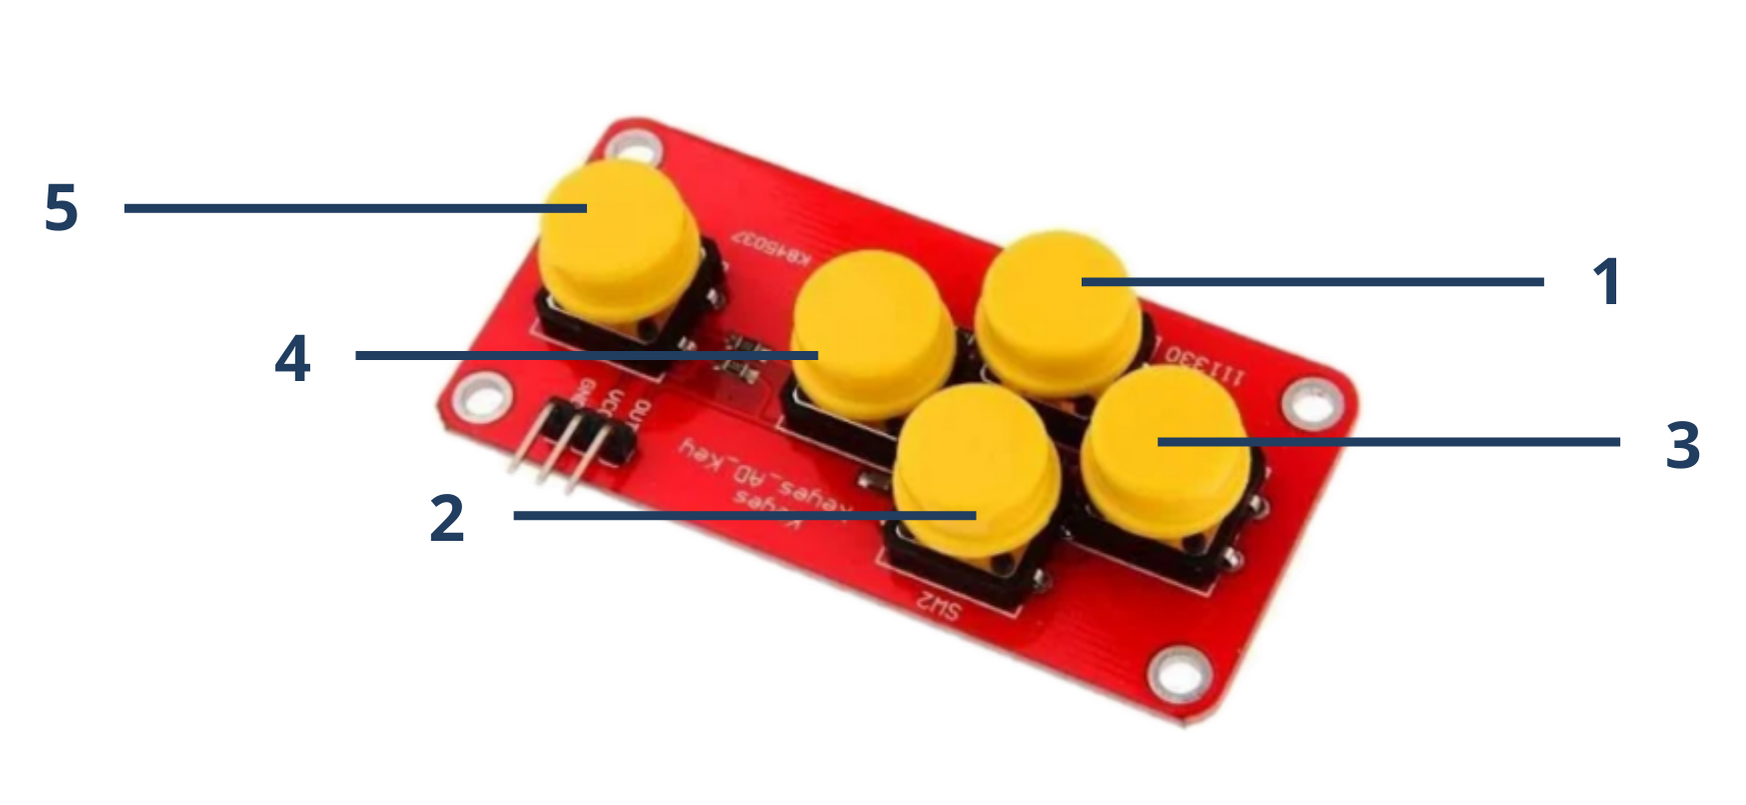
\includegraphics[width=0.6\textwidth]{figuras/eletronica/fotos_componentes/num_teclado.png}}
    \caption{Foto do teclado.} %Identificação do Botão  1- CIMA, 2- BAIXO, 3- DIREITA, 4- ESQUERDA, 5- SELECIONE}
    \label{fig:botoes_identificados}
\end{figure}

O botão 1 tem que subir as telas da interface; o botão 2 descer as telas; o botão 3 muda em telas específicas para direita; o botão 4 para esquerda e; o botão 5 realiza a seleção/\textit{enter} da interface, confirmando e selecionando alguma opção. 

\subsection{Teste do Módulo de Medição e Identificação}

Para o teste deste módulo, é necessário, primeiro, fazer a checagem individual de cada sensor nele contido, onde será avaliado se o sensor não apresenta defeito ao atender os resultados esperados.

Concluída a validação individual de cada sensor, será realizado testes específicos de integração com componentes do módulo de controle em que são conectados, conforme descrito na arquitetura do sistema eletrônico na seção \ref{sec:arq_eletronica}.

\subparagraph*{$\bullet$ Sensor de Temperatura e Umidade - HTU21D} \hfill

A verificação da conexão entre o sensor e o módulo de controle foi explicado anteriormente, na seção de teste do módulo de controle. Para o sensor de temperatura e umidade é realizado o seguinte teste:

\begin{enumerate}
    \item Teste de calibração para ambiente controlado:
    
    \begin{itemize}
        \item \textbf{Objetivo:} Calibrar os valores de temperatura e umidade medidos pelo sensor para um ambiente controlado. Obtendo valores com maior acurácia e precisão que a calibração vinda de fábrica;
        \item \textbf{Itens necessários:} \textit{Raspberry Pi} 4 rodando programa específico para esse teste e ambiente com temperatura variando entre 5 $ ^\circ$C e 55 $^\circ$C;
        \item \textbf{Itens recomendados:} Equipamento externo calibrado que mede temperatura e umidade com precisão igual ou maior;
        \item \textbf{Procedimento:} 
        \begin{enumerate}
            \item Executar o programa de testes para o sensor de temperatura. Esse programa deve capturar os dados do sensor por 5 minutos e armazenar-los para calibração;
            \item Em paralelo a etapa anterior deve ser anotado ou armazenar os dados obtidos pelo equipamento externo de medição;
            \item Analisar os dados obtidos, comparando o sensor com o equipamento externo, e obter os parâmetros de calibração.
            \item Realizar uma segunda medição, seguindo a etapa A, para validar se o objetivo foi alcançado.
        \end{enumerate}
    \end{itemize}

\end{enumerate}

\subparagraph*{$\bullet$ Sensor Fotoelétrico de Barreira} \hfill

Para os sensores fotoelétricos de barreira são realizados os seguintes testes:

\begin{enumerate}
    \item Teste da saída de cada PCI Sensor Fotoelétrico:
    
    \begin{itemize}
        \item \textbf{Objetivo:} Validar a PCI para todas as distâncias entre fotosensores existentes dentro do dispositivo;
        \item \textbf{Itens necessários:} Osciloscópio e bancada de testes com uma plataforma que simula as 5 diferentes distâncias entre o emissor (\textbf{IR333C}) e receptor (\textbf{PT333-3B}) (10,45 mm para contêiner, 66,19 mm para o funil, 55,15 mm para reservatório de copos, 145,28 mm para local de detecção do copo abaixo da câmera e 103,9 mm para porta frontal ou traseira).
        \item \textbf{Procedimento:} 
        \begin{enumerate}
            \item Conexão da PCI com os sensores fotoelétricos para a distância a ser testada na bancada de teste;
            \item Conexão da alimentação e pontas de prova do osciloscópio no terra e saída do comparador da PCI;
            \item Colocar e remover um obstáculo que simula o volume de um comprimido e de um copo entre os sensores fotoelétrico testados na bancada. Realizado várias vezes até ter confiança que funciona para aquela distância;
            \item Repetir o processo para todas as distâncias.
        \end{enumerate}
    \end{itemize}
    
    \item Teste de funcionamento com o módulo de controle:
    
    \begin{itemize}
        \item \textbf{Objetivo:} Validar o funcionamento dos sensores de barreira instalados no dispositivo com o módulo de controle;
        \item \textbf{Itens necessários:} \textit{Raspberry Pi} 4 rodando programa específico para esse teste;
        \item \textbf{Procedimento:} 
        \begin{enumerate}
            \item Instalar os sensores de barreira dentro do dispositivo, seguindo procedimento no manual de montagem no apêndice \ref{manual_montagem};
            \item Executar o programa de teste para os sensores de barreira. Esse programa deve verificar a saída de cada sensor de barreira por um período de 10 segundos, trocando esse intervalo para o próximo até concluir os 30 sensores;
            \item Durante os 10 segundos, que se alterna a colocação e retirada de um obstáculo, é analisado se o módulo de controle está recebendo a resposta apropriada.
        \end{enumerate}
    \end{itemize}

\end{enumerate}

\subparagraph*{$\bullet$ Sensor de Biometria - DY50} \hfill

A verificação da conexão entre o sensor e o módulo de controle foi explicado anteriormente, na seção de teste do módulo de controle. Para o sensor de biometria é realizado os seguintes testes:

\begin{enumerate}
    \item Teste de funcionamento básico do sensor:
    
    \begin{itemize}
        \item \textbf{Objetivo:} Verificar se as funcionalidades básicas de registro, detecção e remoção de impressões digitais estão funcionando.
        \item \textbf{Itens necessários:} \textit{Raspberry Pi} 4 rodando programa específico para esse teste que inclua as bibliotecas do fabricante, conforme descrito no \textit{datasheet};
        \item \textbf{Procedimento:} 
        \begin{enumerate}
            \item Executar o programa de testes para o sensor de biometria;
            \item Realizar o registro de 10 digitais para um único individuo, observando se a validação do programa mostrou que as digitais foram corretamente registradas;
            \item Verificar 10 vezes para cada digital se o programa está reconhecendo-a para o usuário registrado;
            \item Realizar a exclusão da metade das digitais (5), mantendo o restante;
            \item Verificar se as digitais excluídos não são mais reconhecidos pelo programa, conforme esperado;
            \item Verificar se as digitais ainda armazenadas funcionam como antes.
        \end{enumerate}
    \end{itemize}

	\newpage % formatacao
    
    \item Verificação de confiabilidade do registro da digital
    
    \begin{itemize}
        \item \textbf{Objetivo:} Analisar o valor de confiança mínima para o sensor utilizado não considera situações falso-positivas;
        \item \textbf{Itens necessários:} \textit{Raspberry Pi} 4 rodando programa específico para esse teste que inclua as bibliotecas do fabricante, conforme descrito no \textit{datasheet};
        \item \textbf{Procedimento:} 
        \begin{enumerate}
            \item Executar o programa de testes;
            \item Realizar o registro das digitais de pelo menos 5 indivíduos diferentes;
            \item Realizar o procedimento de reconhecimento da digital, coletando os dados de confiança para cada coleta;
            \item Repetir a etapa C várias vezes até concluir um valor ótimo para aplicação no produto.
        \end{enumerate}
    \end{itemize}
\end{enumerate}

\subparagraph*{$\bullet$ Sensor RFID - PN532} \hfill

A verificação da conexão entre o sensor e o módulo de controle foi explicado anteriormente, na seção de teste do módulo de controle. Para o sensor RFID é realizado o seguinte teste:

\begin{enumerate}
    \item Teste de funcionamento da leitura e escrita para as etiquetas dos copos de medicamentos:
    
    \begin{itemize}
        \item \textbf{Objetivo:} Verificar sensor realiza a leitura e escrita da tag RFID na posição padrão dentro do dispositivo;
        \item \textbf{Itens necessários:} \textit{Raspberry Pi} 4 rodando programa específico para esse teste, copo com \textit{tag} RFID instalada;
        \item \textbf{Itens recomendados:} Celular ou dispositivo compatível com a leitura e escrita RFID/NFC da \textit{tag} utilizada;
        \item \textbf{Procedimento:} 
        \begin{enumerate}
            \item Instalar o sensor RFID na posição correta dentro do dispositivo;
            \item Colocar o copo com \textit{tag} RFID na posição onde o sensor irá realizar a leitura;
            \item Executar o programa de testes para o sensor RFID;
            \item Verificar se foi possível realizar a escrita de um ID na etiqueta;
            \item Remover o copo e verificar, com o celular ou dispositivo, se o dado que foi escrito pelo módulo de controle é igual ao que o celular/dispositivo está registrando;
            \item Recolocar o copo na posição anterior e verificar se o sensor RFID consegue realizar a leitura do dado registrado;
            \item Repetir as etapas D, E e F para todos os copos com \textit{tag} RFID.
        \end{enumerate}
    \end{itemize}
\end{enumerate}

\subparagraph*{$\bullet$ Câmera - OV5647} \hfill

A verificação da conexão entre o sensor e o módulo de controle foi explicado anteriormente, na seção de teste do módulo de controle. Para a câmera OV56447 é realizado o seguinte teste:

\begin{enumerate}
    \item Teste de funcionamento da detecção de comprimidos:
    
    \begin{itemize}
        \item \textbf{Objetivo:} Verificar se a qualidade e propriedades das imagens tiradas estão compatíveis com o esperado. Vendo se é possível detectar os comprimidos com o processamento de imagens.
        \item \textbf{Itens necessários:} \textit{Raspberry Pi} 4 rodando programa específico para esse teste, copo, comprimidos registrados no banco de dados para processamento;
        \item \textbf{Procedimento:} 
        \begin{enumerate}
            \item Instalar a câmera na posição correta, dentro do dispositivo;
            \item Colocar o copo com os comprimidos na posição onde a câmera captura os itens no interior;
            \item Executar o programa de testes;
            \item Capturar uma foto com flash do conteúdo no copo;
            \item Analisar aspectos qualitativos da foto, observando a necessidade de ajuste do zoom e intensidade do flash;
            \item Recapturar a imagem e utiliza-la no processamento de imagens;
            \item Verificar se a detecção foi bem sucedida. Caso negativo repetir a calibração até funcionamento correto.
        \end{enumerate}
    \end{itemize}
\end{enumerate}